	\documentclass[11pt,a4paper]{report}
\usepackage{amsmath,geometry,wrapfig,graphicx,float,setspace,hyperref,url,titlesec,apacite,booktabs,bigstrut,nameref,longtable,arydshln,rotating,enumitem,lscape,pgfplots,rotating,mathtools} 
\usepackage{etoolbox}
\usepackage[bottom]{footmisc}
\let\bbordermatrix\bordermatrix
\patchcmd{\bbordermatrix}{8.75}{4.75}{}{}
\patchcmd{\bbordermatrix}{\left(}{\left[}{}{}
\patchcmd{\bbordermatrix}{\right)}{\right]}{}{}
\renewcommand{\rmdefault}{phv} % Arial
\renewcommand{\sfdefault}{phv} % Arial
\usepackage[T1]{fontenc} 
\usepackage{longtable}
\hypersetup{colorlinks=true,citecolor=blue, filecolor=blue, linkcolor=blue, urlcolor=blue}
\numberwithin{figure}{section}
\numberwithin{table}{section}
\numberwithin{equation}{section}
\geometry{top=2.5cm, bottom=2.5cm, left=3.8cm, right=1.9cm}
\bibliographystyle{apacite}
\begin{document}



%----------------------------------------------------------------------------------------
%	TITLE PAGE
%----------------------------------------------------------------------------------------

\begin{titlepage}
\pagenumbering{roman}
\thispagestyle{empty}
\newcommand{\HRule}{\rule{\linewidth}{0.00mm}} 
\center 
%\begin{figure}[H]
%\center{\includegraphics[width=0.5\linewidth]{strathclyde}}
%\end{figure}\vspace{2em}
%{\Large Strathclyde Business School Department of Economics}\\[0.3cm] 
\HRule \\[0.4cm]
{ \huge \bfseries Output Multiplier Analysis}\\[0.4cm] 
\HRule \\[3.5cm]
%{\Large ..... first notes} \\ [4cm] 
{\small Emonts-Holley, T\\Ross, A\\Swales, K} \\ [4cm] 
{\small \today}\\[3cm] % Date
\vfill 
\end{titlepage}


%----------------------------------------------------------------------------------------
%	ABSTRACT
abstract 
IO Type II Multipliers are used widely for economic analysis, but their derivations differ. This paper analyses four methods used to derive the Type II Output Multiplier for the Scottish economy. These methods are measured against the SAM output multiplier in order to determine a best fit. The data for this are predominantly derived from the 2009 Scottish Industry-by-Industry Input-Output Tables and the 2009 Scottish SAM. This paper finds that the use of more comprehensive data for the endogenising of the Household sector results in a closer fit of the Type II in comparison to the SAM output multiplier. However, data availability might limit the computation of the more comprehensive Type II output multiplier.
%----------------------------------------------------------------------------------------

%The content

%----------------------------------------------------------------------------------------
%	DECLARATION  
%----------------------------------------------------------------------------------------

%The content

%----------------------------------------------------------------------------------------
%	WORD COUNT
%----------------------------------------------------------------------------------------

%The content

%----------------------------------------------------------------------------------------
%	ACKNOWLEDGEMENTS  
%----------------------------------------------------------------------------------------

%The content

%----------------------------------------------------------------------------------------
%	TABLE OF CONTENTS / FIGURES  / TABLES
%----------------------------------------------------------------------------------------

\begin{spacing}{1.9}
\tableofcontents 
\end{spacing}
\begin{spacing}{1.9}
\listoffigures
\end{spacing}
\begin{spacing}{1.9}
\listoftables 
\end{spacing}


%----------------------------------------------------------------------------------------
%	END ROMAN
%----------------------------------------------------------------------------------------

\newpage
\setcounter{page}{0} %PN
\pagenumbering{arabic} %PN

%----------------------------------------------------------------------------------------
%	CHAPTERS
%----------------------------------------------------------------------------------------

%% Chapter 1
\chapter{Introduction}
\label{Chapter1}

%%%%%%%%%%%%%%%%%%%%%%%%%%%%%%%%%%%%%%%%%%%%%%%%%%%%%%%%%%
%SECTION
%%%%%%%%%%%%%%%%%%%%%%%%%%%%%%%%%%%%%%%%%%%%%%%%%%%%%%%%%%
\section{Introduction} 
\label{sec:1.1}

Lorem ipsum dolor sit amet, consectetur adipiscing elit. Suspendisse felis velit, ornare ut augue non, ornare rutrum orci. Etiam et eros ligula. Integer iaculis tincidunt purus vel semper. In hac habitasse platea dictumst. Aliquam nec sodales elit. Quisque in accumsan est, eu accumsan urna. Curabitur feugiat faucibus tempor. Sed adipiscing nisi magna, a semper diam ullamcorper et.


%% Chapter 2
\chapter{Social Accounting Matrix for Scotland}
\label{Chapter2}

\section{Introduction} 
\label{sec:2.1}

This chapter outlines the methodology and computations used to construct the 2009 Social Accounting Matrix (SAM) for Scotland. A SAM can be described as a static image (a snapshot) of the flow of goods, services and factors, and the concurrent flow of funds between agents in an economic system for a given time-period \shortcite{Hosoe2010a}. Essentially, the computed SAM extends the Scottish Input Output (IO) tables by incorporating an Income and Expenditure (IncExp) account. Thus, the IncExp account contains information on institutional accounts that is not recorded within the IO tables. Therefore the SAM can be used to analyse social and economic policy in a more comprehensive way. The main benefits and structure of a SAM are outlined in the first sections.  Next, the computed IncExp account and the 2009 Scottish IO tables are combined to complete the 2009 SAM for Scotland. In the last section, the methodology required to compute the IncExp account is described in detail.

%%%%%%%%%%%%%%%%%%%%%%%%%%%%%%%%%%%%%%%%%%%%%%%%%%%%%%%%%%
%SECTION
%%%%%%%%%%%%%%%%%%%%%%%%%%%%%%%%%%%%%%%%%%%%%%%%%%%%%%%%%%
\newpage
\section{Social Accounting Matrices} 
\label{sec:2.2}

The SAM can be considered as an extension to an IO table which not only records macroeconomic-aggregates but also the distribution and redistribution of income. The focus of a SAM therefore lies in recording interrelationships at the meso-level with emphasis on distributive aspects \cite{Keuning1988a}. A SAM can therefore be described as being concerned with the systematic organisation of information about the economic and social structure of a country, region, city or other unit, in a particular time period - usually a year \cite{King1981a}.

\bigskip

In contrast to IO tables, the SAM records flows from producing sectors to factors of production and then on to institutional accounts and finally back to demand for goods \cite{Adelman1986a}. As such, a SAM is different from an IO table as it contains complete information on institutional accounts (i.e. households, government and corporations), instead of solely tracing income and expenditure flows of activities and commodities \shortcite{Breisinger2010a}. The main features of a SAM can be divided into three sections \cite{Round2003a}:   

\bigskip

First, the SAM is a square matrix where the rows represent the flow of goods$/$factors in money terms, whilst the columns represent the flow of payments. The SAM records the expenditures down the columns and the receipts along the rows. The row sums in the SAM show the total receipts and the column sums show the total payments of funds. Importantly, each row sum must equal its corresponding column sum. That is, the total revenue must equal total expenditure in each account \shortcite{Hosoe2010a}. Each cell in the SAM represents a flow of funds from a column account to a row account, thereby documenting the interconnections between these accounts in an explicit way and identifying the source and use of all transactions. 

\bigskip

Second, the SAM is considered to be comprehensive as it shows economic activity in terms of consumption, production, accumulation and distribution (although not necessarily in equivalent detail). 

\bigskip

Third, the SAM is considered to be flexible in the degree of disaggregation, whilst at the same time following a basic accounting framework \shortcite{Breisinger2010a}. The degree of disaggregation generally depends on the motivation behind constructing the SAM (e.g. depending on the location of the initial shock and the outcome variables) and more restrictively, the availability of data \cite{Round2003a}. 

\bigskip

The benefits arising from computing a SAM are multifold. The additional information contained in the SAM, compared to IO tables, can be used to extend and improve the multiplier modelling capacity to include the behaviour of the non-production part of the economy. In particular, the link between activity and changes in household income should improve the Type II multiplier. 

\newpage

Moreover, in contrast to national accounts, the SAM can incorporate a highly disaggregated social breakdown. This is particularly important as a large number of economic interactions happen within the household sector. That is, income from labour and the household sector can be further broken down to analyse distributional effects of policy more accurately \cite{Stuttard2003b}. 

\bigskip

An important side-effect of the compilation process of a SAM is that data gaps and inconsistencies can be identified. This information can be used to improve and extend survey methodologies, definitions and classifications and overall compatibility of data sources \cite{Keuning1988a}. 

\bigskip

The main utility, however, of a SAM is that it provides a comprehensive and consistent record of the interrelationships of an economy at the level of individual production sectors, factors, and institutions. Thereby, the SAM makes available an internally consistent statistical foundation, or benchmark, for the creation of plausible economic models (e.g. Computable General Equilibrium models) which simulate changes to the economy \cite{Reinert1997a}.     

%%%%%%%%%%%%%%%%%%%%%%%%%%%%%%%%%%%%%%%%%%%%%%%%%%%%%%%%%%
%SECTION
%%%%%%%%%%%%%%%%%%%%%%%%%%%%%%%%%%%%%%%%%%%%%%%%%%%%%%%%%%
\newpage
\section{Social Accounting Matrix for Scotland} 
\label{sec:2.3}

The main components of the SAM are the latest Scottish IO tables for Scotland \cite{ScottishGovernment2013a} and the IncExp account. More precisely, the 2009 Industry by Industry (IxI) table for Scotland at basic prices is used. The IxI table is a symmetric IO table with industries (104 industries at SIC07) as the dimension of both rows and columns. Thereby the IxI table records the destination of manufacturing industry outputs. The data on industry linkages can be used to analyse knock-on effects throughout the Scottish economy of a change of final demand \cite{ScottishGovernment2011a}. 

\bigskip

Table \ref{tab:2.3.1} depicts the final SAM that is derived by combining the IxI table and the IncExp account. For illustration several accounts have been aggregated. For example, the 104 industries contained in the SAM are aggregated to one industry (Activities). Thus, it must be emphasises that, for modelling purposes, a more detailed SAM is used.   

\bigskip

As outlined previously, the aggregate 2009 SAM or Scotland is a square matrix with 7 column and 7 row accounts. The rows represent the flow of goods$/$factors in money terms, whilst the columns represent the flow of payments. The SAM records the expenditures down the columns and the receipts along the rows. The row sums in the SAM show the total receipts and the column sums show the total payments of funds. Each row sum equals its corresponding column sum. That is, the total revenue is equal total expenditure in each account. Each cell in the SAM represents a flow of funds from a column account to a row account, thereby documenting the interconnections between these accounts in an explicit way and identifying the source and use of all transactions. 

\bigskip

\begin{table}[H] \caption{Aggregate 2009 SAM for Scotland (in \textsterling million)}
\bigskip \begin{scriptsize} \begin{centering} \begin{doublespacing}
    \begin{tabular}{lrrrrrrrr}
          \toprule
          & \begin{sideways}1. Activities (IOC1-104)\end{sideways} & \begin{sideways}2. Households\end{sideways} & \begin{sideways}3. Corporate\end{sideways} & \begin{sideways}4. Government\end{sideways} & \begin{sideways}5. Capital\end{sideways} & \begin{sideways}6. Employment Income\end{sideways} & \begin{sideways}7. Exports to RUK + ROW\end{sideways} & \begin{sideways}Total (Receipts)\end{sideways} \bigstrut\\
    \hline
    1. Activities (IOC1-104) & 63,607 & 49,802 & -     & 29,486 & 13,981 & -     & 54,045 & 210,920 \\
    2. Households & -     & -     & \textbf{15,104} & \textbf{25,124} & -     & 63,561 & \textbf{4,088} & 107,877 \\
    3. Corporate & -     & \textbf{6,931} & -     & \textbf{34,647} & -     & -     & \textbf{11,928} & 53,507 \\
    4. Government & 43,221 & \textbf{27,947} & \textbf{5,248} & \textbf{16,861} & 1,495 & -     & \textbf{20,363} & 115,136 \\
    5. Capital & -     & \textbf{5,070} & \textbf{24,826} & \textbf{119}   & -     & -     & \textbf{-10,086} & 19,930 \\
    6. Employment Income & 63,561 & -     & -     & -     & -     & -     & -     & 63,561 \\
    7. Imports from RUK + ROW & 40,532 & \textbf{18,126} & \textbf{8,328} & \textbf{8,898} & \textbf{4,455} & -     & 10,470 & 90,808 \\
\bottomrule 
\end{tabular}%  
\bigskip \begin{flushright} Cells derived from the IncExp Account are \textbf{highlighted}. Remaining stem directly from the 2009 IxI table \cite{ScottishGovernment2013a}.\end{flushright} \label{tab:2.3.1} 
\end{doublespacing} \end{centering} \end{scriptsize} \end{table} \bigskip

The first row of the SAM, for example, can be read as follows: raw material purchases of goods within Scotland (\textsterling63,607m), Household consumption expenditure on goods$/$services (\textsterling49,802m), Government current expenditure (\textsterling29,486m), investment expenditure on Scottish goods (\textsterling13,981m), exports to RUK + ROW (\textsterling54,045m) and the total of \textsterling210,920m represents total aggregate demand of gross outputs.

\bigskip 

Extending the IO table by incorporating the IncExp accounts yields a SAM with the following entries (the * indicated that entries, with the exception of the IncExp extension, were directly taken from the IO table):

\bigskip

\begin{itemize}
    \item Activities are directly taken from the IO table and contains the 104 industries at SIC07. Activities show the destination of manufacturing industry outputs, including manufacturing products or other secondary products.
    \item Households are directly taken from the IO table* and is the sum of the Household account and the Non-Profit Institutions Serving Households (NPISHs) account in the IO table.
    \item Corporate is solely derived within the IncExp account, thereby providing a more complete record of the institutional account. 
    \item Government is directly taken from the IO table* and is the sum of the Central and Local Government accounts in the IO table.
    \item Capital is directly taken from the IO table* from Gross fixed capital formation (GFCF).
    \item Employment income is taken directly from the IO table*.
    \item Exports$/$imports to and from RUK$/$ROW (including good $/$ services and transfers) are directly taken from the IO table* RUK and ROW exports$/$imports entry.
\end{itemize}

\bigskip

Importantly, constructing the SAM by extending IO tables by means of an IncExp account does not require any rebalancing (e.g. total receipts per account match total expenditures). That is, the IO table is fully incorporated without the need of changing any entries thereof. All cells that were added to the IO table to compute the SAM are balanced within the IncExp account so that total revenue equal total expenditure in each account. This approach incorporates the IO tables at face value, assuming that the data therein are the best possible estimates of Scottish data. Each account in the Scottish SAM is balanced by their corresponding account. So for example, Government expenditures (\textsterling115,136m) are balanced by Government receipts (\textsterling115,136m). 

\bigskip

It must be emphasised again that the SAM is meant to fit around the existing IO tables and other national statistics. Data necessary for the construction of the SAM that are not contained within the IO table are derived by computing an IncExp account. This account records income and expenditure of households, corporations, government, capital and the external sector in detail. The construction of the IncExp account is outlined in the following section.

%%%%%%%%%%%%%%%%%%%%%%%%%%%%%%%%%%%%%%%%%%%%%%%%%%%%%%%%%%
%SECTION
%%%%%%%%%%%%%%%%%%%%%%%%%%%%%%%%%%%%%%%%%%%%%%%%%%%%%%%%%%
\newpage
\section{The Income and Expenditure Accounts for 2009}
\label{sec:2.4}

The Income and Expenditure Accounts provide a details on the flow of funds for the main three local transactors (Households, Corporations and Government) as well as for the Capital and External Accounts. The Accounts are compiled using publicly available data, including both UK and Scottish Government data as well as figures from the 2009 IO Tables for Scotland. The IncExp Accounts are internally consistent, which ensures that the SAM is automatically balanced. The above section outlined the role that the IncExp Accounts have in extending the IO Tables into a SAM for Scotland. This section provides an overview of how the IncExp Accounts are constructed and the following section gives a detailed breakdown of how each entry in the Accounts is calculated. First in this section, the layout of the Accounts is presented. Second, the data calculation and internal balancing is discussed. Third, the data sources used for the Accounts are  


\subsection{Layout}
\label{sec:2.4.1}

The IncExp Accounts (see Table \ref{tab:2.4.1}) are divided into five different sectors (Households, Corporations, Government, Capital and External) and they also give the Scottish Trade and External Balance with both RUK and ROW. Each of those sectors is divided further into an Income and an Expenditure part, hence the name for these Accounts. Each cell can be identified either through the name, e.g. Corporations > Income > Profit Income (OVA) or through the equivalent number code, 19 in this case. The latter method is used when cross-referencing in the detailed breakdown of the cells in the Methodology section (\ref{sec:2.5}).Every sector has a Total Income and a Total Expenditure Figure, which is a summation of the entries in each section (highlighted in bold). The Household and Government sector have additional Control Totals from external sources and therefore they are presented with two Totals. The Primary Sectors (Household, Corporations and Government) have a similar cell breakdown with Income/Payments to the other Primary Sectors as well as External Transfer payments making up the biggest share of entries. Additionally, all Primary Sectors have a Profit Income (OVA) entry and a Payments to Capital entry on the Income and on the Expenditure side, respectively. Cells with one star following the numerical entry refer to Balancing Items and those with two stars refer to Corresponding Figures. A detailed discussion of those entries can be found in Calculation Overview and Internal Balancing (\ref{sec:2.4.2}).


% % % % % % % % % % % % % % % % % % % % % % % % % % % % % % % % %
% % % % % % THE INCOME AND EXPENDITURE ACCOUNTS TABLE % % % % % %
% % % % % % % % % % % % % % % % % % % % % % % % % % % % % % % % %


\begin{table}[H] \caption{Income-Expenditure Accounts for Scotland (in \textsterling million)}
\bigskip \begin{scriptsize} \begin{centering} \begin{spacing}{1.2}
    \begin{tabular}{lrllrl}
          \toprule
    \textbf{HOUSEHOLDS} \bigstrut\\
    \hline  
\bigstrut[t]    1. \textbf{Income} & \textbf{107877} & & 10. \textbf{Expenditure} & \textbf{107877} & \\
    2. Income from Employment & 63561  &   & 11. IO Expenditure & 74138 & \\
    3. Profit Income (OVA) & 5289 & & 12. Payments to Corporations & 6931 &* \\
    4. Income from Corporations & 15104 & & 13. Payments to Government & 21379 & \\
    5. Income from Government & 19835 & & 14. Transfers to ROW & 119 & \\
    6. Transfers from RUK & 1852 & & 15. Transfers to RUK & 238 & \\
    7. Transfers from ROW & 2237 & & 16. Payments to Capital (Savings) & 5070 &\\
    8. \textbf{Total Household Income} & \textbf{107877} & & 17. \textbf{Total Expenditure} & \textbf{107877} & \\
    9. \textbf{Mixed and Prop Income Unalloc.} & 0 & \bigstrut[b]\\
    \hline
\bigstrut[t]    \textbf{CORPORATIONS} \bigstrut\\
    \hline
\bigstrut[t] 18. \textbf{Income} & \textbf{53507}  &   & 24. \textbf{Expenditure} & \textbf{53507} & \\
       19. Profit Income (OVA) & 29456 & & 25. Payments to Households & 15104 &** \\
       20. Income from Households & 6931 &** & 26. Payments to Government & 5248 & \\
       21. Income from Government & 5191 &** & 27. Transfers to RUK & 3768 & \\
       22. Income from RUK & 5964 & & 28. Transfers to ROW & 4560 & \\
       23. Income from ROW & 5964 & & 29. Payments to Capital (Savings) & 24826 &* \\
    \hline
    \textbf{GOVERNMENT} \bigstrut\\
    \hline
\bigstrut[t]       30. \textbf{Income} & \textbf{63530}  &   & 37. \textbf{Expenditure} & \textbf{63530} & \\
       31. Profit Income (OVA) & 3697 & & 38. IO Expenditure & 30017 & * \\
       32. Net Commodity Taxes & 13165 & & 39. Payments to Corporations & 5191 &* \\
       33. Income from Households & 21379 &** & 40. Payments to Households & 19835 &** \\
       34. Income from Corporations & 5248 &** & 41. Transfers to RUK & 8368 & \\
       35. Income from RUK & 20041 &* & 42. Payments to Capital (Savings) & 119 & \\
       36. \textbf{Total Govt Inc Balancing Total} & \textbf{63530} &** & 43. \textbf{Total Govt Exp Balancing Total} & \textbf{63530} &  \\ 
    \hline
    \textbf{CAPITAL} \bigstrut\\
    \hline
\bigstrut[t]       44. \textbf{Income} & \textbf{19930}  &   & 49. \textbf{Expenditure} & \textbf{19930} & \\
       45. Households & 5070 &** & 50. IO Expenditure & 19930 &  \\
       46. Corporations & 24826 &** &  \\
       47. Government & 119 &** &  \\
       48. RUK/ROW & -10086 &** &  \\ 
    \hline
    \textbf{EXTERNAL} \bigstrut\\
    \hline
\bigstrut[t]  51. RUK Income from Scotland & 67133  &   & 58. RUK Expenditure in Scotland & 70595 & \\
       52. Goods \& Services & 54759 & & 59. Goods \& Services & 42739 & \\
       53. Transfers & 12374 & & 60. Transfers & 27857 & \\
       54. RUK Income from Scotland & 23676 & & 61. ROW Expenditure in Scotland & 27378 & \\
       55. Goods \& Services & 18997 & & 62. Goods \& Services & 19178 & \\
       56. Transfers & 4679 & & 63. Transfers & 8201 & \\
       & & & 64. Tourist Expenditure in Scotland & 2921 & \\
       57. \textbf{Total Income} & \textbf{90808} & & 65. \textbf{Total Expenditure} & \textbf{100894} &  \\  
        & & & 66. Surplus/Deficit &-10086 & \\   
    \hline
    \textbf{G\&S TRADE BALANCE} \bigstrut\\
    \hline
\bigstrut[t] \quad \enspace \thinspace Scotland with RUK and ROW & &   & \quad \enspace \thinspace Total Balance of Payments & & \\
       67. RUK & -12020 & & 69. RUK & 5215 &  \\
       68. ROW & 181 & & 70. ROW & 4871 & \\
       & & & 71. Total Balance of Payments & 10086 & \\  
    \hline    
    \textbf{EXTERNAL BALANCE} \bigstrut\\
    \hline
\bigstrut[t]   72. Income from Employment & -3462 & & & & \\
       73. Profit Income (OVA) & -3703 & & & &  \\
       74. Income from Corporations & -2921 & & & & \\
       75. Income from Government & -10086 & & & & \\ 
    \hline
    \hline    
\qquad \qquad \qquad Balancing Item: *   & & & Row Entries (Element determines Column)  \\ 
\qquad \qquad \qquad Corresponding Figure: ** & & & Row Entries (Element determines Column)  \bigstrut\\       
          \hline            
    \bottomrule
\end{tabular}%  
\bigskip \begin{flushright}\end{flushright} \label{tab:2.4.1}
\end{spacing} \end{centering}  \end{scriptsize} \end{table}


\subsection{Calculation Overview and Internal Balancing}
\label{sec:2.4.2}

Most of the figures in the Accounts are calculated using either figures from the IO Tables or external sources. The references for each calculation are both in the Methodology Section  (\ref{sec:2.5}) as well as within the SAM file. Most governmental data is issued in the financial year format, i.e. April of year one until end of March of year 2. In order to get data for the calendar year 2009, which is also the format of the IO Tables, a one-quarter share of the year one data is taken and a three-quarter share of year two (1/4*2008/09 + 3/4*2009/10). Using the updated 2006 SAM, the data sources for each IncExp Account entry are updated and when possible more accurate sources/figures are used in the calculation of the 2009 Accounts.
Some cells, however, are not calculated using the above-mentioned sources. First, some cells are Balancing Items, denoted with one star (see Table \ref{tab:2.4.1}). These entries are derived by taking the Totals of the relevant account and deducting the sum of all other entries, but the one marked as a Balancing Item. The reason for this methodology is two-fold. On the one hand, in order to balance the Total Income and the Total Expenditure of the Primary Sectors, at least one entry needs to absorb any deviation in the balance between income and expenditure. On the other hand, for some cells the data availability or quality is simply not there and thus those entries with the least robust data are chosen to be Balancing Items. The Balancing Items further ensure the internal consistency of the IncExp Accounts and therefore the SAM balances automatically once the IO Tables are extending through these Accounts. Second, there are cells denoted with two stars and these are the Corresponding Figures. Due to the assumption of the Circular Flow of the Economy, where the income that a receives from b is equal to the payment that b makes to a, some entries are equal to the figures derived for other cells. For example, the Payments to Government made by Corporations (cell 26) is equal to the Income from Corporations received by the Government. Further, all Income entries for the Capital Accounts are Corresponding Figures, as these are equal to the Payments to Capital entries by each of the Primary Sector as well as the net External balance (cell 66). 


\subsection{Data}
\label{sec:2.4.3}

The data used in the construction of the IncExp Accounts is all taken from either UK or Scottish Government sources and is publicly available. Figure \ref{fig:2.4.1} shows how much data is derived from the main data sources. For this, each component of the IncExp cells is deconstructed. For example, some cells use one figure from the IO Tables, one from GERS (Government Expenditure and Revenue Scotland) and one from the HM Treasury. This would give three separate sources which would be counted as individual entries and then the total of those entries' is used to calculate the shares allocated to each source of data origin. Note, that when data is given in financial year format, there are technically two entries from that source, which is then transformed into a calendar year entry, as outlined above. However, this is then taken as a single entry for the calculation of the shares here, as it would otherwise skew the percentages. As Figure \ref{fig:2.4.1} shows the three biggest sources for data used in the IncExp Acounts are GERS (30\%), ONS (29\%) and the 2009 IO Tables (24\%). The figure highlights the large reliance on UK Government sources, which is over a third of all data entries. In order to transform this data for the Scottish IncExp Accounts, various shares are used \footnote{Shares are Scottish over total UK values}. There are three different shares, which are all close in total value, however, theoretical considerations favour different shares for certain data as is outlined here. First, the GDP share (8.22\%) is used for example for Dividend Payments both Private and Public. Second, the population share (8.41\%) applies to UK Government spending on behalf of the Scottish public, for instance. Third, the households share is used, for example, for RUK Transfer Payments to Scotland. Although the use of the shares transforms the data sufficiently for the calculation of the Accounts, improving the availability of Scottish data for all of income or expenditure in Scotland would result in more accurate figures for the IncExp Accounts and the 2009 SAM for Scotland. Nevertheless, the quality of the data used for the IncExp Accounts is of the highest quality, since it is taken from Scottish and UK governmental publications. 


\begin{figure}[!htbp]
  \begin{center}
       \ifpdf
         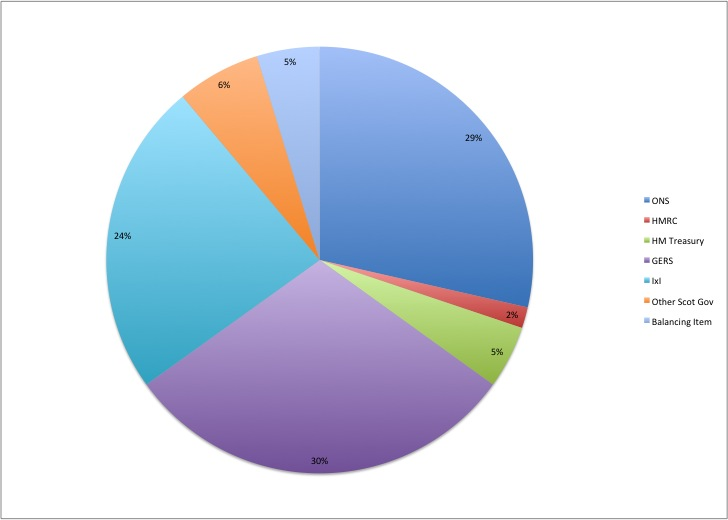
\includegraphics[height=4.3in,width=6in]{incexpsources}
       \else
         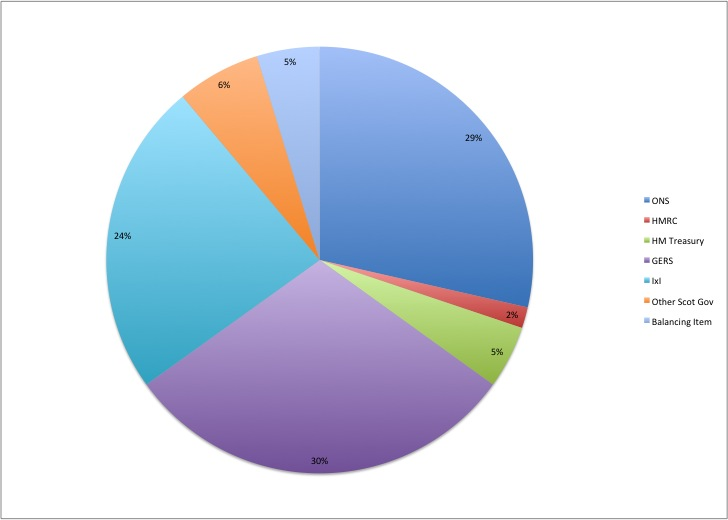
\includegraphics[bb = 92 86 545 742, height=6in]{incexpsources}
       \fi
    \caption{Percentage of data sources in Income and Expenditure Accounts}
    \label{incexpsources}
  \end{center} \label{fig:2.4.1}
\end{figure}


\pagebreak

\pagebreak


%%%%%%%%%%%%%%%%%%%%%%%%%%%%%%%%%%%%%%%%%%%%%%%%%%%%%%%%%%
%SECTION
%%%%%%%%%%%%%%%%%%%%%%%%%%%%%%%%%%%%%%%%%%%%%%%%%%%%%%%%%%
\newpage
\section{Income and Expenditure Accounts - Methodology}
\label{sec:2.5}

\bigskip
\begin{center}
\textbf{\LARGE Households}
\end{center}

\begin{enumerate}


\item \textbf {Income}

\bigskip

The Household income entry is derived from the latest revised figures of Scottish Gross Disposable Household Income (GDHI) for 2009 \cite{ONS2013a}. This data is obtained for Scotland at NUTS2 level covering the variables listed in Table \ref{tab:2.4.1}. The total Household Income figure of \textsterling107,877m is obtained by summing up Operating surplus$/$Mixed income (\textsterling9,437m), Compensation of employees (\textsterling64,645m), Property income received minus paid (\textsterling8,485m - \textsterling551m), Imputed social contributions$/$Social benefits received (\textsterling23,559m), and Other current transfers received minus Other current transfers paid (\textsterling5,102m - \textsterling2,800m).    

\bigskip

\begin{table}[H] \caption{Scottish Gross Disposable Household Income (GDHI) in \textsterling million by component}
\bigskip \begin{scriptsize} \begin{centering} \begin{doublespacing}
% INSERT
    \begin{tabular}{lr}
    \toprule
    Operating surplus$/$Mixed income &          9,437  \bigstrut[t]\\
    Compensation of employees &        64,645  \\
    Property income, received &          8,485  \\
    Primary resources total &        82,566  \bigstrut[b]\\
    Property income, paid &             551  \bigstrut[t]\\
    Primary uses total &             551  \\
    Balance of primary incomes &        82,015  \\
    Imputed social contributions/Social benefits received &        23,559  \bigstrut[b]\\
    Other current transfers, received &          5,102  \bigstrut[t]\\
    Secondary resources total &        28,663  \\
    Current taxes on income, wealth etc. &        13,893  \\
    Social contributions/Social benefits paid &        17,678  \bigstrut[b]\\
    Other current transfers, paid &          2,800  \bigstrut[t]\\
    Secondary uses total &        34,370  \\
    Balance of secondary income & -        5,708  \\
    Gross Disposable Income &        76,307  \bigstrut[b]\\
\bottomrule \end{tabular}%  
\bigskip \begin{flushright} Data sourced from: \cite{ONS2013a}\end{flushright} \label{tab:2.5.1} 
\end{doublespacing} \end{centering} \end{scriptsize} \end{table} \bigskip

\bigskip




\begin{equation}
\begin{split}
\text{Income} =
\text{Total Household Income}_\text{GDHI}
\end{split} \label{eq:2.5.1}
\end{equation}

\begin{equation} \nonumber
110677 = 110677
\end{equation}\\

\item \textbf {Income from Employment}

This is the ``Total intermediate demand'' \text{|| }``Compensation of employees'' from the IO Tables. [Source: Scottish Government (2013a)] \cite{ScottishGovernment2013a}

\begin{equation}
\begin{split}
\text{Income from Employment} =  \\ \\
(\text{Total Intermediate Demand}\|\text{Compensation of Employees})
\end{split} \label{eq:2.5.2}
\end{equation}

\begin{equation} \nonumber
63561 = 63561
\end{equation}\\


\item \textbf {Profit Income (OVA)}

\bigskip

This entry requires that the Gross Operating Surplus for Scotland is identified. Yet, as shown in Table \ref{tab:2.4.1}, data for Scotland is only available as an aggregate comprising of Operating surplus and Mixed income equal in total to \textsterling9,437m. Therefore, this figure has to be disaggregated to identify the Gross Operating Surplus component. This is estimated by using shares derived from 1999 GDHI data which reports these figures individually. There are no alternative datasets available that would allow for a better estimation of Scottish Gross Operating Surplus for 2009. 

\bigskip

Table \ref{tab:2.5.2} illustrates this process. First, the GDHI data for 1999 is obtained \shortcite{Hermannsson2010a}. Next, the the GDHI components are listed. Last, using the Gross Operating Surplus and Gross mixed income shares derived from 1999, the 2009 figures are disaggregated (i.e. \textsterling9437m * (\textsterling3413m / \textsterling3413m + \textsterling2677m) = \textsterling5289m and \textsterling9437 * (\textsterling2677m / \textsterling2677m + \textsterling3413m) = \textsterling4148m). This process yields the required Gross Operating Surplus estimate for Scotland of \textsterling5,289m. Thus, 2009 data (the control total) is disaggregate by using 1999 shares to yield the necessary variables.      

\bigskip

\begin{table}[H] \caption{Scottish Gross Disposable Household Income (GDHI) in \textsterling million by component}
\bigskip \begin{scriptsize} \begin{centering} \begin{doublespacing}
% INSERT
    \begin{tabular}{lrrr}
        \toprule
          & 1999  & 2009  & 2009 using shares \\
        \hline      
    Total household income &              71,296  &               107,877  &               107,877  \\
    Gross operating surplus &                 3,413  &                   9,437  &                   5,289  \\
    Gross mixed income &                 2,677  &   -    &                   4,148  \\
    Compensation of employees &              40,593  &                 64,645  &                 64,645  \\
    Net property income &                 6,591  &                   7,934  &                   7,934  \\
    All pensions &                 8,961  &                 23,559  &                 13,886  \\
    Other social benefits &                 6,242  &   -    &                   9,673  \\
    Net other income &                 2,820  &                   2,302  &                   2,302  \\
    \hline
    Total household disposable income &              48,931  &                 76,307  &                 76,307  \\
\bottomrule \end{tabular}%  
\bigskip \begin{flushright} Data sourced from: \cite{ONS2013a} and \shortcite{Hermannsson2010a}\end{flushright} \label{tab:2.4.2} 
\end{doublespacing} \end{centering} \end{scriptsize} \end{table} \bigskip



\begin{equation}
\begin{split}
\text{Profit Income} = \text{Gross Operating Surplus}_\text{GDHI}
\end{split} \label{eq:2.5.3}
\end{equation}

\begin{equation} \nonumber
5289 = 5289
\end{equation}\\


\item \textbf {Income from Corporations}

This is calculated from three sources. First, taking the Capital Gains Tax receipts as presented in GERS and dividing it by the fixed 18\% Capital Gains Tax Rate for 2008-10 gives an estimate of the actual monetary value of the capital gain received by Scottish households for 2009. 
Second, the total income received by households from corporations is added. This comprises multiplying the share of Scottish GDP, which is calculated using the ratio of total UK GDP at market prices over Scottish GDP at market prices, by the Total of ``UK Private Dividends'' paid out by private non-financial corporations in the UK. In turn this figure is then multiplied by the average (figures are only available for 2008 and 2010) of an individual`s share of total equity on a UK basis, which is used to distinguish the dividend payments received by private shareholders versus, for example, funds. Further, the total income figure is comprised of adding an estimate of the ``Total Private Pensions'' received by Scottish households to the above as well as household`s ``Net Other Income'' from the GDHI. 
Third, the unallocated income from 10 is added in order to balance this part of the Accounts.  \cite{ScotGov2013b,HMRC2013,ONS2011c,ONS2012}


\begin{equation}
\begin{split}
\text{Income from Corporations} =  \\ \\
\text{Total Household Income from Corporations}\\
+\text{Household Income from Capital Gains}\\
+\text{Mixed and Prop Income Unallocated}_\text{IncExp}\\
\end{split} \label{eq:2.5.4}
\end{equation}

\begin{equation} \nonumber
17904 = 15558+1478+869
\end{equation}

\begin{center}
\line(1,0){250}
\end{center}

\textit{where}

\begin{equation} 
\begin{split}
\text{Total Household Income from Corporations} = \\ 
(\text{Scottish GDP Share}*\text{Total UK Private Dividend Payments})\\
*(\text{Individual Share of Total Equity} + \text{Total Private Pension}\\
 + \text{Net Other Income})
\end{split} \label{eq:2.5.5}
\end{equation} 

\begin{equation} \nonumber
15558 = (8.22\% * 85816)*((\frac{10.2\%+11.5\%}{2})+9691+5102)
\end{equation}

\begin{center}
\line(1,0){250}
\end{center}


\begin{equation} 
\begin{split}
\text{Household Income from Capital Gains} = \\ 
(1/4 *\text{Households' Captial Gains Tax Payments}_\text{08-09}\\
+ 3/4 *\text{Households' Captial Gains Tax Payments}_\text{09-10})\\
\div \text{Capital Gains Tax Rate}
\end{split} \label{eq:2.5.6}
\end{equation} 

\begin{equation} \nonumber
1478 = (1/4*572+3/4*164)\div 18\%
\end{equation}

\begin{center}
\line(1,0){250}
\end{center}


\begin{equation} 
\begin{split}
\text{Mixed and Prop Income Unallocated} = \\ 
(\text{Total Household Income}_\text{GDHI}-\text{Total Household Income}_\text{IncExp})\\
\end{split} \label{eq:2.5.7}
\end{equation} 

\begin{equation} \nonumber
869 = 110677-109808
\end{equation}\\

\item \textbf {Income from Government}

The first part of this figure is the annualised ``Social Protection Payments'' to Scottish households and the second one is the ``Public Dividend Payments'' received by Scottish households. The latter is calculated in accordance with the methodology outlined above for ``Private Dividend Payments''. The dividend payments are sourced from non-financial corporations, Central Government and Local Government accounts and are multiplied by the Scottish GDP share as well as the average individual`s share of total equity and further multiplied by the UK Public Dividend payments.  \cite{ScotGov2013b,ONS2011c}

\begin{equation}
\begin{split}
\text{Income from Government} =  \\ \\
(1/4*\text{Total Social Protection}_\text{08-09}\\
+3/4*\text{Total Social Protection}_\text{09-10})\\
+(\text{Scottish GDP Share} \\
*(\text{UK Public Dividends}_\text{Non-Financial Corporations}\\
+\text{UK Public Dividends}_\text{Central Government}\\
+\text{UK Public Dividends}_\text{Local Government})\\
*((\text{Individual's Share of Total Equity}_\text{2008}\\
+\text{Individual's Share of Total Equity}_\text{2009})\div 2))
\end{split} \label{eq:2.5.8}
\end{equation}


\begin{equation} \nonumber
\begin{split}
19835 = (1/4*18653+3/4*20193)\\
+(8.22\%*(25+2214+772)*((10.2\%+11.5\%)\div 2))
\end{split}
\end{equation}\\


\item \textbf {Transfers from RUK}

These transfers are calculated by first, taking the total figure of dividends paid to Scottish households. This figure is calculated by using the share of Scottish Households of total UK Households and multiplying it by ``Total RUK Dividends'' paid to households. The latter figure is based on the average individual`s share of total equity multiplied by the difference between Total UK- and Total Scottish- private dividends in order to obtain the RUK dividend payments to Households in Scotland. 
Second, this is then added to the difference of the ``Compensation of Employees'' according to the GDHI estimates and the actual figure of income from employment as calculated for the Income and Expenditure Account (see 2).
\cite{ONS2011c,ONS2011a,ONS2011b}


\begin{equation}
\begin{split}
\text{Transfers from RUK} =  \\ \\
\text{Total RUK Dividends to Scottish Households}\\
+(\text{Compensation of Employees}_\text{GDHI}\\
-\text{Income from Employment}_\text{IncExp})
\end{split} \label{eq:2.5.9}
\end{equation}

\begin{equation} \nonumber
1852 = 767+(64645-63561)
\end{equation}\\

\begin{center}
\line(1,0){250}
\end{center}

\textit{where}

\begin{equation}
\begin{split}
\text{Total RUK Dividends to Scottish Households}=\\
\text{Scottish Household Share}*\text{Total RUK Dividends to Households}
\end{split} \label{eq:2.5.10}
\end{equation}

\begin{equation}\nonumber
767=8.98\%*8546
\end{equation}


\item \textbf {Transfers from ROW}

The first part of this figure is calculated by multiplying UK employment income from ROW with the OVA for Scotland (see below for breakdown of OVA and OVA repatriated calculations). Added to this is the Scottish share of UK GDP (as shown above) multiplied with the Scottish household share of OVA for UK property and entrepreneurial income and multiplied by the actual amount of the ``UK Property and Entrepreneurial Income''. \cite{ScotGov2013a,ONS2011c,ScotGov2013b}

\begin{equation}
\begin{split}
\text{Transfers from ROW} =  \\ \\
(\text{Scottish Share of UK Total OVA}*\\
\text{UK Employment Income from ROW})\\
+(\text{Scottish Household OVA}*\text{Scottish GDP Share of UK}\\
*\text{UK Property and Entrepreneurial Income})
\end{split} \label{eq:2.5.11}
\end{equation}


\begin{equation} \nonumber
2237 = (143588.31\%)+(169313*15\%*8.22\%)
\end{equation}\\

\item \textbf {Total Household Income}

Totals Figure: Summation of all of the above, excluding the total household income figure obtained from the GDHI (sum: 2 to 7).

\begin{equation}
\begin{split}
\text{Total Household Income} =  \\ \\
(\text{Income from Employment}^\text{Households}_\text{IncExp}\\
+\text{Profit Income (OVA)}^\text{Households}_\text{IncExp}\\
+\text{Income from Corporations}^\text{Households}_\text{IncExp}\\
+\text{Income from Government}^\text{Households}_\text{IncExp}\\
+\text{Transfers from RUK}^\text{Households}_\text{IncExp}\\
+\text{Transfers from ROW}^\text{Households}_\text{IncExp})
\end{split} \label{eq:2.5.12}
\end{equation}

\begin{equation} \nonumber
110677 = 63561+5289+17904+19835+1852+2237
\end{equation}\\


\item \textbf {Mixed and Prop Income Unallocated}

Balancing item equal to the difference of Household Income as presented in the GDHI and the sum of all income figures derived above. This figure gets added into the Income from Corporations as outlined above and is thus zero, due to the two household income figures balancing now. [Source: IncExp Accounts] \cite{ONS2011b}

\begin{equation}
\begin{split}
\text{Income Unallocated} =  \\ \\
\text{Income}^\text{Households}_\text{IncExp}\\
-\text{Income from Employment}^\text{Households}_\text{IncExp}
\end{split} \label{eq:2.5.13}
\end{equation}


\begin{equation} \nonumber
869 = 110677-109808
\end{equation}\\


\pagebreak

\item \textbf {Expenditure}

Totals Figure: Summation of figures presented below, from IO Expenditure to Transfers to ROW (sum: 11 to 16).

\begin{equation}
\begin{split}
\text{Expenditure} =  \\ \\
(\text{IO Expenditure}^\text{Households}_\text{IncExp}\\
+\text{Payments to Corporations}^\text{Households}_\text{IncExp}\\
+\text{Payments to Government}^\text{Households}_\text{IncExp}\\
+\text{Payments to Capital}^\text{Households}_\text{IncExp}\\
+\text{Transfers from RUK}^\text{Households}_\text{IncExp}\\
+\text{Transfers from ROW}^\text{Households}_\text{IncExp})
\end{split} \label{eq:2.5.14}
\end{equation}

\begin{equation} \nonumber
110677 = 74138+9600+21379+5202+238+119
\end{equation}\\


\item \textbf {IO Expenditure}

This cell is made up of ``Households'' and ``Non-Profit Institutions Serving Households'' (NPISHs) – ``Total intermediate consumption at basic prices'' as well as ``Taxes less subsidies on products'' for both sectors. \cite{ScotGov2013a}

\begin{equation}
\begin{split}
\text{IO Expenditure} =  \\ \\
(\text{Final Cons. Expend.}_\text{Households}\|\text{Total Interm. Cons.})\\
+(\text{Final Cons. Expend.}_\text{NPISH}\|\text{Total Interm. Cons.})\\
+(\text{Final Cons. Expend.}_\text{Households}\|\text{Taxes less subsidies on products})\\
+(\text{Final Cons. Expend.}_\text{NPISH}\|\text{Taxes less subsidies on products})
\end{split} \label{eq:2.5.15}
\end{equation}

\begin{equation} \nonumber
74138 = 64890+6568+26803+0
\end{equation}\\


\item \textbf {Payments to Corporations}

Balancing Item: which takes the Total Expenditure and subtracts from it the IO Expenditure, Payments to Government, Payments to Capital, Transfers to RUK and Transfers to ROW (17 – 11,14,15,16).

\begin{equation}
\begin{split}
\text{Payments to Corporations} =  \\ \\
\text{Total Expenditure}^\text{Households}_\text{IncExp}-\text{Transfers to ROW}^\text{Households}_\text{IncExp}\\
-\text{Transfers to RUK}^\text{Households}_\text{IncExp}-\text{Payments to Capital}^\text{Households}_\text{IncExp}\\
-\text{Payments to Government}^\text{Households}_\text{IncExp}-\text{IO Expenditure}^\text{Households}_\text{IncExp}
\end{split} \label{eq:2.5.16}
\end{equation}

\begin{equation} \nonumber
9600 = 110677-119-238-5202-21379-74138
\end{equation}\\


\item \textbf {Payments to Government}

This refers to the annualised tax payments by Scottish households. These taxes are: Income Tax, Capital Gains Tax, Inheritance Tax, Stamp Duties, Half Insurance Premium Tax, Council Tax and Social Security Contributions (NI). \cite{ScotGov2013b}

\begin{equation}
\begin{split}
\text{Payments to Government} =  \\ \\
(1/4*(\text{Income Tax}_\text{08-09}+\text{Capital Gains Tax}_\text{08-09}\\
+(\text{Inheritance Tax}_\text{08-09}+\text{Stamp Duties}_\text{08-09}\\
+(\text{Half Insurance Premium Tax}_\text{08-09}+\text{Council Tax}_\text{08-09}\\
+(\text{Social Security Contributions}_\text{08-09}))\\
+(3/4*(\text{Income Tax}_\text{09-10}+\text{Capital Gains Tax}_\text{09-10}\\
+(\text{Inheritance Tax}_\text{09-10}+\text{Stamp Duties}_\text{09-10}\\
+(\text{Half Insurance Premium Tax}_\text{09-10}+\text{Council Tax}_\text{09-10}\\
+(\text{Social Security Contributions}_\text{09-10}))\\
\end{split} \label{eq:2.5.17}
\end{equation}

\begin{equation} \nonumber
\begin{split}
21379=(1/4*(10642+572+178+594+96+1960+7992))\\
+(3/4*(10364+164+146+516+95+1961+7915))
\end{split}
\end{equation}\\


\item \textbf {Transfers to RUK}

The value of Transfers to ROW (16) is multiplied by two.

\begin{equation}
\begin{split}
\text{Transfers to RUK} =  \\ \\
\text{Transfers to ROW}^\text{Households}_\text{IncExp}*2
\end{split} \label{eq:2.5.18}
\end{equation}

\begin{equation} \nonumber
238 = 119*2
\end{equation}\\


\item \textbf {Transfers to ROW}

This figure is made up of the amount of employee compensation that is paid to the ROW, i.e. the part that is deducted from GDP in order to arrive at GNP figures, times the share of Scottish OVA of Corporate Income (\ref{eq:2.5.84}). \cite{ONS2011c}

\begin{equation}
\begin{split}
\text{Transfers to ROW} =  \\ \\
\text{UK Payments to ROW}*\text{Scottish Corporate Income OVA}
\end{split} \label{eq:2.5.19}
\end{equation}

\begin{equation} \nonumber
119 = 1435*8.31\%
\end{equation}\\


\item \textbf {Payments to Capital (Savings)}

The Total Expenditure (18) is multiplied by the Household Saving rate as given by SNAP, in order to obtain an estimate for this cell. \cite{ScotGov2013c}

\begin{equation}
\begin{split}
\text{Payments to Capital} =  \\ \\
\text{Total Household Income}^\text{Households}_\text{IncExp}\\
+\text{Household Savings Rate}_\text{SNAP}
\end{split} \label{eq:2.5.20}
\end{equation}

\begin{equation} \nonumber
5202 = 110677*0.047
\end{equation}\\


\item \textbf {Total Expenditure}

Corresponding Figure: Equal to the Total Household Income (9).

\begin{equation}
\begin{split}
\text{Total Expenditure} =  \\ \\
\text{Total Household Income}^\text{Households}_\text{IncExp}
\end{split} \label{eq:2.5.21}
\end{equation}

\begin{equation} \nonumber
110677 = 110677
\end{equation}\\



\pagebreak

\begin{center}
\textbf{\LARGE Corporations}
\end{center}

\item \textbf {Income}

Totals Figure: Equal to all of the items below in this section (19 to 23).

\begin{equation}
\begin{split}
\text{Income} =  \\ \\
\text{Profit Income}^\text{Corporations}_\text{IncExp}\\
+\text{Income from Households}^\text{Corporations}_\text{IncExp}\\
+\text{Income from Government}^\text{Corporations}_\text{IncExp}\\
+\text{Income from RUK}^\text{Corporations}_\text{IncExp}\\
+\text{Income from ROW}^\text{Corporations}_\text{IncExp}
\end{split} \label{eq:2.5.22}
\end{equation}

\begin{equation} \nonumber
56175 = 29456+9600+5191+5964+5964
\end{equation}\\

\item \textbf {Profit Income (OVA)}

Taking the ``Total Intermediate Demand'' – ``Gross Operating Surplus'', the OVA of both Households and Government (3 and 31) are deducted from it from it.  \cite{ScotGov2013a,ONS2011b}

\begin{equation}
\begin{split}
\text{Profit Income} =  \\ \\
\text{Total Intermediate Demand}\|\text{Gross Operating Surplus}\\
-\text{Profit Income}^\text{Households}_\text{IncExp}-\text{Profit Income}^\text{Government}_\text{IncExp}
\end{split} \label{eq:2.5.23}
\end{equation}

\begin{equation} \nonumber
29456 = 38441-5289-3697
\end{equation}\\


\item \textbf {Income from Households}

Corresponding Figure: Equal to Payments to Corporations under Household Expenditure (12).

\begin{equation}
\begin{split}
\text{Income from Households} =  \\ \\
\text{Payments to Corporations}^\text{Households}_\text{IncExp}
\end{split} \label{eq:2.5.24}
\end{equation}

\begin{equation} \nonumber
9600 = 9600
\end{equation}\\


\item \textbf {Income from Government}

Corresponding Figure: Equal to Payments to Corporations under Government Expenditure (39).

\begin{equation}
\begin{split}
\text{Income from Government} =  \\ \\
\text{Payments to Corporations}^\text{Government}_\text{IncExp}
\end{split} \label{eq:2.5.25}
\end{equation}

\begin{equation} \nonumber
5191 = 5191
\end{equation}\\


\item \textbf {Income from RUK}

Using the Scottish share of UK property and entrepreneurial income (see \ref{eq:2.5.82}), it is multiplied by the corporate share of OVA. One half of this figure is used for this cell and the other for the one below (23). \cite{ONS2011c}

\begin{equation}
\begin{split}
\text{Income from RUK} =  \\ \\
1/2*\text{Corporate OVA Share}\\
*\text{Scottish Share of UK Property and Entrepreneurial Income}
\end{split} \label{eq:2.5.26}
\end{equation}

\begin{equation} \nonumber
5964 = 84.8\%*14070*1/2
\end{equation}\\


\item \textbf {Income from ROW}

Other half of figure calculated in first part of 22.

\begin{equation}
\begin{split}
\text{Income from RUK} =  \\ \\
1/2*\text{Corporate OVA Share}\\
*\text{Scottish Share of UK Property and Entrepreneurial Income}
\end{split} \label{eq:2.5.27}
\end{equation}

\begin{equation} \nonumber
5964 = 84.8\%*14070*1/2
\end{equation}\\


\pagebreak

\item \textbf {Expenditure}

Totals Figure: cells below (25 to 29).

\begin{equation}
\begin{split}
\text{Expenditure} =  \\ \\
\text{Payments to Households}^\text{Corporations}_\text{IncExp}\\
+\text{Payments to Government}^\text{Corporations}_\text{IncExp}\\
+\text{Transfers to RUK}^\text{Corporations}_\text{IncExp}\\
+\text{Transfers to ROW}^\text{Corporations}_\text{IncExp}\\
+\text{Payments to Capital}^\text{Corporations}_\text{IncExp}
\end{split} \label{eq:2.5.28}
\end{equation}

\begin{equation} \nonumber
56175 = 17904+5248+3768+4560+24695
\end{equation}\\


\item \textbf {Payments to Households}

Corresponding Figure: Equal to Household Income from Corporations (4).

\begin{equation}
\begin{split}
\text{Payments to Households} =  \\ \\
\text{Income from Corporations}^\text{Households}_\text{IncExp}
\end{split} \label{eq:2.5.29}
\end{equation}

\begin{equation} \nonumber
17904 = 17904
\end{equation}\\


\item \textbf {Payments to Government}

These are the annualised corporate taxes: Corporation Tax, (Windfall Tax) Half Insurance Premium Tax, Landfill Tax, Non-Domestic Rates, Other Taxes and Royalties, Interest and Dividends \cite{ScotGov2013b}

\begin{equation}
\begin{split}
\text{Payments to Government} =  \\ \\
(1/4*(\text{Corporation Tax}_\text{08-09}+\text{Half Insurance Premium Tax}_\text{08-09}\\
+(\text{Landfill Tax}_\text{08-09}+\text{Non-Domestic Rates}_\text{08-09}\\
+(\text{Other Taxes and Royalties}_\text{08-09}+\text{Interest and Dividends}_\text{08-09}\\
+(3/4*(\text{Corporation Tax}_\text{09-10}+\text{Half Insurance Premium Tax}_\text{09-10}\\
+(\text{Landfill Tax}_\text{09-10}+\text{Non-Domestic Rates}_\text{09-10}\\
+(\text{Other Taxes and Royalties}_\text{09-10}+\text{Interest and Dividends}_\text{09-10}\\
\end{split} \label{eq:2.5.30}
\end{equation}

\begin{equation} \nonumber
\begin{split}
5248 = (1/4*(2841+96+82+1736+250+608))\\
+(3/4(2680+95+85+1822+212+233))
\end{split}
\end{equation}\\


\item \textbf {Transfers to RUK}

Equal to OVA repatriated to RUK (see \ref{eq:2.5.80}). \cite{ScotGov2012}\\

\begin{equation}
\begin{split}
\text{Transfers to RUK} =  \\ \\
\text{Share of OVA Repatriated to RUK}*\text{Profit Income}^\text{Corporations}_\text{IncExp}
\end{split} \label{eq:2.5.31}
\end{equation}

\begin{equation} \nonumber
3768 = 13\%829456
\end{equation}\\


\item \textbf {Transfers to ROW}

Equal to OVA repatriated to ROW (see \ref{eq:2.5.81}). \cite{ScotGov2012}

\begin{equation}
\begin{split}
\text{Transfers to ROW} =  \\ \\
\text{Share of OVA Repatriated to ROW}*\text{Profit Income}^\text{Corporations}_\text{IncExp}
\end{split} \label{eq:2.5.32}
\end{equation}

\begin{equation} \nonumber
4560 = 15\%*829456
\end{equation}\\


\item \textbf {Payments to Capital (Savings)}

Balancing Item: This figure is derived by summing up the ``Gross Fixed Capital Formation'' (GFCF) for all Public Sectors in the IO Tables and then deducting the sum of the ``Taxes less subsidies on production'' for these sectors. The Public Sectors are: Water and Sewerage, Public Administration and Defence, Education, Health, Residential Care and Social Work. \cite{ScotGov2013a}

\begin{equation}
\begin{split}
\text{Payments to Capital} =  \\ \\
\text{Income}^\text{Corporations}_\text{IncExp}\\
-\text{Payments to Households}^\text{Corporations}_\text{IncExp}\\
-\text{Payments to Government}^\text{Corporations}_\text{IncExp}\\
-\text{Transfers to RUK}^\text{Corporations}_\text{IncExp}\\
-\text{Transfers to ROW}^\text{Corporations}_\text{IncExp}
\end{split} \label{eq:2.5.33}
\end{equation}

\begin{equation} \nonumber
24695 = 56175-17904-5248-3768-4560
\end{equation}\\


\pagebreak

\begin{center}
\textbf{\LARGE Government}
\end{center}

\item \textbf {Income}

Totals Figure: Sum of cells below (31 to 35).

\begin{equation}
\begin{split}
\text{Income} =  \\ \\
\text{Profit Income}^\text{Government}_\text{IncExp}\\
+\text{Net Commodity Tax}^\text{Government}_\text{IncExp}\\
+\text{Income from Households}^\text{Government}_\text{IncExp}\\
+\text{Income from Corporations}^\text{Government}_\text{IncExp}
\end{split} \label{eq:2.5.34}
\end{equation}

\begin{equation} \nonumber
63530 = 3697+13165+21379+5248+10041
\end{equation}\\


\item \textbf {Profit Income (OVA)}

Equal to ``Taxes less subsidies on production'' for all public sectors (see 30).  \cite{ScotGov2013a}

\begin{equation}
\begin{split}
\text{Profit Income} =  \\ \\
\text{Water and Sewerage}\|\text{Gross Operating Surplus}\\
+\text{Public Administration and Defence}\|\text{Gross Operating Surplus}\\
+\text{Education}\|\text{Gross Operating Surplus}\\
+\text{Health}\|\text{Gross Operating Surplus}\\
+\text{Residential Care}\|\text{Gross Operating Surplus}\\
+\text{Social Work}\|\text{Gross Operating Surplus}
\end{split} \label{eq:2.5.35}
\end{equation}

\begin{equation} \nonumber
3697 = 710+865+463+817+590+253
\end{equation}\\


\item \textbf {Net Commodity Taxes}

This cell is the sum of ``Total Intermediate Deman''” – ``Taxes less subsidies on production'' and ``Total Demand for Products'' – ``Taxes less subsidies on products''. \cite{ScotGov2013a}\\

\begin{equation}
\begin{split}
\text{Net Commodity Taxes} =  \\ \\
\text{Total Intermediate Demand}\|\text{Taxes less Subsidies on Production}\\
+\text{Total Demand for Products}\|\text{Taxes less Subsidies on Products}\\
\end{split} \label{eq:2.5.36}
\end{equation}

\begin{equation} \nonumber
13165 = 1232+11933
\end{equation}\\


\item \textbf {Income from Households}

Corresponding Figure: Equal to Payments to Government under Household Expenditure (13).

\begin{equation}
\begin{split}
\text{Income from Households} =  \\ \\
\text{Payments to Government}^\text{Households}_\text{IncExp}
\end{split} \label{eq:2.5.37}
\end{equation}

\begin{equation} \nonumber
21379 = 21379
\end{equation}\\


\item \textbf {Income from Corporations}

Corresponding Figure: Equal to Payments to Government under Corporations Expenditure (26).

\begin{equation}
\begin{split}
\text{Income from Coporations} =  \\ \\
\text{Payments to Government}^\text{Corporations}_\text{IncExp}
\end{split} \label{eq:2.5.38}
\end{equation}

\begin{equation} \nonumber
5248 = 5248
\end{equation}\\


\item \textbf {Income from RUK}

Balancing Item: Total Gov. Income Balancing Total (36) minus the sum of Profit Income, Net Commodity Taxes, Income from Households and Income from Corporations (31 to 34).\\

\begin{equation}
\begin{split}
\text{Income from RUK} =  \\ \\
\text{Total Government Income Balancing}\\
-\text{Profit Income}^\text{Government}_\text{IncExp}\\
-\text{Net Commodity Taxes}^\text{Government}_\text{IncExp}\\
-\text{Income from Households}^\text{Government}_\text{IncExp}\\
-\text{Income from Corporations}^\text{Government}_\text{IncExp}
\end{split} \label{eq:2.5.39}
\end{equation}

\begin{equation} \nonumber
20041 = 63530-3697-13165-21379-5248
\end{equation}\\


\item \textbf {Total Government Income Balancing Total}

Corresponding Figure: Equal to Total Government Expenditure Balancing Total (43).\\

\begin{equation}
\begin{split}
\text{Total Government Income} =  \\ \\
\text{Total Government Expenditure Balancing Total}^\text{Government}_\text{IncExp}
\end{split} \label{eq:2.5.40}
\end{equation}

\begin{equation} \nonumber
63530 = 63530
\end{equation}\\



\pagebreak

\item \textbf {Expenditure}

Totals Figure: Summation for cells below (38 to 42).\\

\begin{equation}
\begin{split}
\text{Expenditure} =  \\ \\
\text{IO Expenditure}^\text{Government}_\text{IncExp}\\
+\text{Payments to Corporations}^\text{Government}_\text{IncExp}\\
+\text{Payments to Households}^\text{Government}_\text{IncExp}\\
+\text{Transfers to RUK}^\text{Government}_\text{IncExp}\\
+\text{Payments to Capital}^\text{Government}_\text{IncExp}
\end{split} \label{eq:2.5.41}
\end{equation}

\begin{equation} \nonumber
63530 = 30017+5191+19835+8368+119
\end{equation}\\


\item \textbf {IO Expenditure}

This is the ``Central Government'' and ``Local Governments'' – ``Total intermediate consumption at basic prices''. \cite{ScotGov2013a}

\begin{equation}
\begin{split}
\text{IO Expenditure} =  \\ \\
\text{Central Government}\|\text{Total Intermediate Consumption at basic Prices}\\
+\text{Local Government}\|\text{Total Intermediate Consumption at basic Prices}
\end{split} \label{eq:2.5.42}
\end{equation}

\begin{equation} \nonumber
30017 = 19462+10555
\end{equation}\\


\item \textbf {Payments to  Corporations}

Balancing Item:  Total Government Expenditure Balancing Total (44) minus IO Expenditure, Payments to Households, Transfers to RUK and Payments to Capital (Savings) (38, 40, 41, 42).

\begin{equation}
\begin{split}
\text{Payments to Corporations} =  \\ \\
\text{Total Government Expenditure Balancing Total}^\text{Government}_\text{IncExp}\\
-\text{IO Expenditure}^\text{Government}_\text{IncExp}\\
+\text{Payments to Households}^\text{Government}_\text{IncExp}\\
+\text{Transfers to RUK}^\text{Government}_\text{IncExp}\\
+\text{Payments to Capital}^\text{Government}_\text{IncExp}
\end{split} \label{eq:2.5.43}
\end{equation}

\begin{equation} \nonumber
5191 = 63530-30017-19835-8368-119
\end{equation}\\


\item \textbf {Payments to Households}

Corresponding Figure: Income from Government from the Household Income Accounts (5).\\

\begin{equation}
\begin{split}
\text{Payments to Households} =  \\ \\
\text{Income from Government}^\text{Households}_\text{IncExp}
\end{split} \label{eq:2.5.44}
\end{equation}

\begin{equation} \nonumber
19835 = 19835
\end{equation}\\


\item \textbf {Transfers to RUK}

This is the annualised estimated non-identifiable Government Expenditure, which is based on the Scottish population share of the UK Total non-identifiable public spending. \cite{ScotGov2013b}

\begin{equation}
\begin{split}
\text{Transfers to RUK} =  \\ \\
1/4*\text{Estimated Non-Identifiable Expenditure}_\text{08-09}\\
+3/4\text{Estimated Non-Identifiable Expenditure}_\text{09-10}
\end{split} \label{eq:2.5.45}
\end{equation}

\begin{equation} \nonumber
8368 = 1/4*8174+3/4*8432
\end{equation}\\


\item \textbf {Payments to Capital (Savings)}

This is the sum of ``Gross Fixes Capital Formation'' for all Public Sectors, which is then subtracted by ``Taxes less subsidies on production'' for these sectors. \cite{ScotGov2013a}\\

\begin{equation}
\begin{split}
\text{Payments to Capital} =  \\ \\
(\text{Gross Fixed Capital Formation}\|\text{Water and Sewerage}\\
+\text{Gross Fixed Capital Formation}\|\text{Public Administration and Defence}\\
+\text{Gross Fixed Capital Formation}\|\text{Education}\\
+\text{Gross Fixed Capital Formation}\|\text{Health}\\
+\text{Gross Fixed Capital Formation}\|\text{Residential Care}\\
+\text{Gross Fixed Capital Formation}\|\text{Social Work})\\
-(\text{Water and Sewerage}\|\text{Taxes less Subsidies on Production}\\
+\text{Public Administration and Defence}\|\text{Taxes less Subsidies on Production}\\
+\text{Education}\|\text{Taxes less Subsidies on Production}\\
+\text{Health}\|\text{Taxes less Subsidies on Production}\\
+\text{Residential Care}\|\text{Taxes less Subsidies on Production}\\
+\text{Social Work}\|\text{Taxes less Subsidies on Production})
\end{split} \label{eq:2.5.46}
\end{equation}

\begin{equation} \nonumber
\begin{split}
119 = (1+174+7+0+0+1)\\
-(28+0+18+11+3+4)
\end{split}
\end{equation}\\


\item \textbf {Total Government Expenditure Balancing Total}

This is the annualised ``Total Identifiable Expenditure'' of the Scottish Government plus the non-identifiable estimate (see 41). Then, the annualised ``Total managed expenditure'', ``Total Identifiable''- and ``Total non-identifiable Expenditure'' of the UK is multiplied by the Scottish population share of the UK Total population and then taken off the two former sums of Public Sector spending in Scotland. \cite{HMTR2012,ONS2011a}\\

\begin{equation}
\begin{split}
\text{Total Government Expenditure} =  \\ \\
(1/4 * \text{Total Identifiable Expenditure}_{08-09} \\
+ 3/4 * \text{Total Identifiable Expenditure}_{09-10})\\
+ (1/4 * \text{Total Non-Identifiable Expenditure}_{08-09} \\
+ 3/4 * \text{Total Non-Identifiable Expenditure}_{09-10}) \\
( 1/4 * \text{Scot. Pop. Share} * ( \text{Total Man. Exp.}^{UK}_{08-09} \\
- \text{Total Ident. Exp.}^{UK}_{08-09} \\
- \text{Total Man. Non-Ident.}^{UK}_{08-09})) \\
( 1/4 * \text{Scot. Pop. Share} * ( \text{Total Man. Exp.}^{UK}_{09-10} \\
- \text{Total Ident. Exp.}^{UK}_{09-10} \\
- \text{Total Man. Non-Ident.}^{UK}_{09-10}))
\end{split} \label{eq:2.5.47}
\end{equation}


\begin{equation} \nonumber
\begin{split}
63530 = (1/4*(50779+8174))+(3/4*(53617+8432))\\
+(1/4*8.41\%*(629745-515734-87697))\\
+(3/4*8.41\%*(670150-559134-84021))
\end{split}
\end{equation}\\


\pagebreak


\begin{center}
\textbf{\LARGE Capital}
\end{center}

\item \textbf {Income}

Totals Figure: Sum of cells below (45 to 48).

\begin{equation}
\begin{split}
\text{Income} =  \\ \\
\text{Households}^\text{Capital}_\text{IncExp}\\
+\text{Corporations}^\text{Capital}_\text{IncExp}\\
+\text{Government}^\text{Capital}_\text{IncExp}\\
+\text{RUK/ROW}^\text{Capital}_\text{IncExp}
\end{split} \label{eq:2.5.48}
\end{equation}

\begin{equation} \nonumber
19930 = 5202+24695+119+(-10086)
\end{equation}\\


\item \textbf {Households)}

Corresponding Figure: Payments to Capital of the Household Expenditure Account (14).

\begin{equation}
\begin{split}
\text{Households} =  \\ \\
\text{Payments to Capital}^\text{Households}_\text{IncExp}
\end{split} \label{eq:2.5.49}
\end{equation}

\begin{equation} \nonumber
5202 = 5202
\end{equation}\\


\item \textbf {Corporate}

Corresponding Figure: Payments to Capital (savings) of the Corporation Expenditure Account (29).

\begin{equation}
\begin{split}
\text{Corporate} =  \\ \\
\text{Payments to Capital}^\text{Corporations}_\text{IncExp}
\end{split} \label{eq:2.5.50}
\end{equation}

\begin{equation} \nonumber
24695 = 24695
\end{equation}\\


\item \textbf {Government}

Corresponding Figure: Payments to Capital (savings) of the Government Expenditure Account (42).

\begin{equation}
\begin{split}
\text{Government} =  \\ \\
\text{Payments to Capital}^\text{Government}_\text{IncExp}
\end{split} \label{eq:2.5.51}
\end{equation}

\begin{equation} \nonumber
119 = 119
\end{equation}\\


\item \textbf {RUK/ROW}

Corresponding Figure: Surplus/Deficit of the External Expenditure Account (66).

\begin{equation}
\begin{split}
\text{RUK/ROW} =  \\ \\
\text{Total Income}^\text{External}_\text{IncExp}\\
-\text{Total Expenditure}^\text{External}_\text{IncExp}
\end{split} \label{eq:2.5.52}
\end{equation}

\begin{equation} \nonumber
-10086 = 90808-100894
\end{equation}\\


\pagebreak

\item \textbf {Expenditure}

Corresponding Figure: IO Expenditure (50).
    
\begin{equation}
\begin{split}
\text{Expenditure} =  \\ \\
\text{IO Expenditure}^\text{Capital}_\text{IncExp}
\end{split} \label{eq:2.5.53}
\end{equation}

\begin{equation} \nonumber
19930 = 19930
\end{equation}\\


\item \textbf {IO Expenditure}

This is the sum of ``Total Gross Capital Formation'' – ``Total intermediate consumption at basic prices'' and ``Total Gross Capital Formation'' – ``Taxes less subsidies on products''. \cite{ScotGov2013a}

\begin{equation}
\begin{split}
\text{IO Expenditure} =  \\ \\
\text{Total Gross Capital Formation}\|\text{Total Interm. Consumption at Basic Prices}\\
+\text{Total Gross Capital Formation}\|\text{Taxes Less Subsidies on Products}
\end{split} \label{eq:2.5.54}
\end{equation}

\begin{equation} \nonumber
19930 = 18453+1495
\end{equation}\\



\pagebreak


\begin{center}
\textbf{\LARGE External}
\end{center}

\item \textbf {UK Income from Scotland}

Totals Figure: This is the sum of the two cells below: Goods \& Services and Transfers (52 \& 53).\\

\begin{equation}
\begin{split}
\text{UK Income from Scotland} =  \\ \\
\text{Goods \& Services}^\text{External}_\text{IncExp}\\
+\text{Transfers}^\text{External}_\text{IncExp}
\end{split} \label{eq:2.5.55}
\end{equation}

\begin{equation} \nonumber
67133 = 54759+12374
\end{equation}\\


\item \textbf {Goods \& Services}

This is the “Total Demand for Products” from RUK. \cite{ScotGov2013a}

\begin{equation}
\begin{split}
\text{Goods \& Services} =  \\ \\
\text{Total Demand for Products}\|\text{Imports from Rest of UK}
\end{split} \label{eq:2.5.56}
\end{equation}

\begin{equation} \nonumber
54759 = 54759
\end{equation}\\


\item \textbf {Transfers}

This is the sum of: ``Transfers to RUK'' from the Household Expenditure Account, ``Transfers to RUK'' from the Corporations Expenditure Account and the ``Transfers to RUK'' from the Government Expenditure Account (6, 22, 35).\\

\begin{equation}
\begin{split}
\text{Transfers} =  \\ \\
\text{UK Income from Scotland} =  \\ \\
\text{Transfers to RUK}^\text{Households}_\text{IncExp}\\
+\text{Transfers to RUK}^\text{Corporations}_\text{IncExp}\\
+\text{Transfers to RUK}^\text{Government}_\text{IncExp}
\end{split} \label{eq:2.5.57}
\end{equation}

\begin{equation} \nonumber
12374 = 238+3768+8368
\end{equation}\\


\item \textbf {ROW Income from Scotland}

Totals Figure: This is the sum of the two cells below: Goods \& Services and Transfers (55 \& 56).\\

\begin{equation}
\begin{split}
\text{ROW Income from Scotland} =  \\ \\
\text{Goods \& Services}^\text{External}_\text{IncExp}\\
+\text{Transfers}^\text{External}_\text{IncExp}
\end{split} \label{eq:2.5.58}
\end{equation}

\begin{equation} \nonumber
23676 = 18997+4697
\end{equation}\\


\item \textbf {Goods \& Services}

This is the ``Total Demand for Products'' – ``ROW''. \cite{ScotGov2013a}

\begin{equation}
\begin{split}
\text{Goods \& Services} =  \\ \\
\text{Total Demand for Products}\|\text{Imports from ROW}
\end{split} \label{eq:2.5.59}
\end{equation}

\begin{equation} \nonumber
18997 = 18997
\end{equation}\\


\item \textbf {Transfers}

This is the sum of: ``Transfers to ROW'' from the Household Expenditure Account and ``Transfers to ROW'' from the Corporations Expenditure Account (7 \& 23).\\

\begin{equation}
\begin{split}
\text{Transfers} =  \\ \\
\text{Transfers to ROW}^\text{Households}_\text{IncExp}\\
+\text{Transfers to RUK}^\text{Corporations}_\text{IncExp}
\end{split} \label{eq:2.5.60}
\end{equation}

\begin{equation} \nonumber
4679 = 119+4560
\end{equation}\\


\item \textbf {Total Income}

Totals Figure: This is the sum of the two cells above: ``UK income from Scotland'' and ``ROW income from Scotland'' (51 \& 54).\\

\begin{equation}
\begin{split}
\text{Total Income} =  \\ \\
\text{UK Income from Scotland}^\text{External}_\text{IncExp}\\
+\text{ROW Income from Scotland}^\text{External}_\text{IncExp}
\end{split} \label{eq:2.5.61}
\end{equation}

\begin{equation} \nonumber
90808 = 67133+23676
\end{equation}\\



\pagebreak

\item \textbf {UK Expenditure in Scotland}

Totals Figure: This is the sum of the two cells below: Goods \& Services and Transfers (59 \& 60).\\

\begin{equation}
\begin{split}
\text{UK Expenditure in Scotland} =  \\ \\
\text{Goods \& Services}^\text{External}_\text{IncExp}\\
+\text{Transfers}^\text{External}_\text{IncExp}
\end{split} \label{eq:2.5.62}
\end{equation}

\begin{equation} \nonumber
70595 = 42739+27857
\end{equation}\\


\item \textbf {Goods \& Services}

This is the ``Total intermediate consumption at basic prices'' – ``Rest of UK exports''. \cite{ScotGov2013a}\\

\begin{equation}
\begin{split}
\text{Goods \& Services} =  \\ \\
\text{Rest of UK Exports}\|\text{Total Interm. Consumption at Basic Prices}
\end{split} \label{eq:2.5.63}
\end{equation}

\begin{equation} \nonumber
42759 = 42759
\end{equation}\\


\item \textbf {Transfers}

This is the sum of: ``Transfers from RUK'' from the Household Income Account, ``Income from RUK'' from the Corporations Income Account and ``Income from RUK'' from the Government Income Account (15, 27, 41).

\begin{equation}
\begin{split}
\text{Transfers} =  \\ \\
\text{Transfers from RUK}^\text{Households}_\text{IncExp}\\
+\text{Income from RUK}^\text{Corporations}_\text{IncExp}\\
+\text{Income from RUK}^\text{Government}_\text{IncExp}
\end{split} \label{eq:2.5.64}
\end{equation}

\begin{equation} \nonumber
27857 = 1852+5964+20041
\end{equation}\\


\item \textbf {ROW Expenditure in Scotland}

Totals Figure: This is the sum of the two cells below: Goods \& Services and Transfers.

\begin{equation}
\begin{split}
\text{ROW Expenditure in Scotland} =  \\ \\
\text{Goods \& Services}^\text{External}_\text{IncExp}\\
+\text{Transfers}^\text{External}_\text{IncExp}
\end{split} \label{eq:2.5.65}
\end{equation}

\begin{equation} \nonumber
27378 = 19178+8201
\end{equation}\\


\item \textbf {Goods \& Services}

This is the ``Total intermediate consumption at basic prices'' – ``Rest of world exports''. \cite{ScotGov2013a}

\begin{equation}
\begin{split}
\text{Goods \& Services} =  \\ \\
\text{Rest of World Exports}\|\text{Total Interm. Consumption at Basic Prices}
\end{split} \label{eq:2.5.66}
\end{equation}

\begin{equation} \nonumber
19178 = 19178
\end{equation}\\


\item \textbf {Transfers}

This is the sum of: ``Transfers from ROW'' from the Household Income Account and ``Income from ROW'' from the Corporations Income Account (16 \& 28).

\begin{equation}
\begin{split}
\text{Transfers} =  \\ \\
\text{Transfers from ROW}+\text{Income from ROW}
\end{split} \label{eq:2.5.67}
\end{equation}

\begin{equation} \nonumber
8201 = 2237+5964
\end{equation}\\



\item \textbf {Tourist Expenditure in Scotland}

This is the sum of the ``Non-resident household expenditure in Scotland'' (under ``Final consumption expenditure'') - ``Total intermediate consumption at basic prices'' and ``Taxes less subsidies on products''. \cite{ScotGov2013a}

\begin{equation}
\begin{split}
\text{Tourist Expenditure in Scotland} =  \\ \\
\text{Final Consumption Expenditure Non-Resident}\\
\text{Household Expenditure in Scotland}\\
\|\text{Total Interm. Consumption at Basic Prices}\\
\text{Final Consumption Expenditure Non-Resident}\\
\text{Household Expenditure in Scotland}\\
\|\text{Taxes Less Subsidies on Products}
\end{split} \label{eq:2.5.68}
\end{equation}

\begin{equation} \nonumber
2921 = 2599+322
\end{equation}\\


\item \textbf {Total Expenditure}

This is the sum of the above cells: ``UK expenditure in Scotland'', ``ROW expenditure in Scotland'' and ``Tourist expenditure in Scotland''.

\begin{equation}
\begin{split}
\text{Total Expenditure} =  \\ \\
\text{UK Expenditure in Scotland}^\text{External}_\text{IncExp}\\
+\text{ROW Expenditure in Scotland}^\text{External}_\text{IncExp}\\
+\text{Tourist Expenditure in Scotland}^\text{External}_\text{IncExp}
\end{split} \label{eq:2.5.69}
\end{equation}

\begin{equation} \nonumber
100894 = 70595+27378+2921
\end{equation}\\


\item \textbf {Surplus/Deficit}

This is the balance of the External Accounts’ ``Total income'' minus ``Total expenditure'' (57 - 65).

\begin{equation}
\begin{split}
\text{Surplus/Deficit} =  \\ \\
\text{Total Income}^\text{External}_\text{IncExp}\\
-\text{Total Expenditure}^\text{External}_\text{IncExp}
\end{split} \label{eq:2.5.70}
\end{equation}

\begin{equation} \nonumber
-10086 = 90808-100894
\end{equation}\\



\pagebreak


\begin{center}
\textbf{\LARGE Goods and Services Trade Balance}
\end{center}

\item \textbf {RUK}

This is the balance of the ``Goods and Services'' of ``UK expenditure in Scotland'' minus those of ``UK income from Scotland'' (59 - 51).

\begin{equation}
\begin{split}
\text{Goods \& Services Trade Balance with RUK} =  \\ \\ 
\text{RUK Goods \& Services Expenditure in Scotland}^\text{External}_\text{IncExp}\\
-\text{RUK Goods \& Services Income from Scotland}^\text{External}_\text{IncExp}
\end{split} \label{eq:2.5.71}
\end{equation}

\begin{equation} \nonumber
-12020 = 42739-54759
\end{equation}\\


\item \textbf {ROW}

This is the balance of the ``Goods and Services'' of ``ROW expenditure in Scotland'' minus those of ``ROW income from Scotland'' (62 - 55).

\begin{equation}
\begin{split}
\text{Goods \& Services Trade Balance with ROW} =  \\ \\ 
\text{ROW Goods \& Services Expenditure in Scotland}^\text{External}_\text{IncExp}\\
-\text{ROW Goods \& Services Income from Scotland}^\text{External}_\text{IncExp}
\end{split} \label{eq:2.5.72}
\end{equation}

\begin{equation} \nonumber
181 = 19178-18997
\end{equation}\\



\pagebreak

\item \textbf {RUK}

Taking the ``UK expenditure in Scotland'' from the External Accounts, the ``Tourist expenditure in Scotland'' is added to it. This is then multiplied by the share attributed to UK versus ROW tourist and subsequently subtracted by ``UK income from Scotland'' (58,64,51).  \cite{ONS2010a}\\

\begin{equation}
\begin{split}
\text{Total Balance of Payments RUK} =  \\ \\
\text{RUK Expenditure in Scotland}^\text{External}_\text{IncExp}\\
+(\text{RUK Share of Tourist Expenditure in Scotland}\\
*\text{Tourist  Expenditure in Scotland}^\text{External}_\text{IncExp})\\
-\text{RUK Income from Scotland}^\text{External}_\text{IncExp}
\end{split} \label{eq:2.5.73}
\end{equation}

\begin{equation} \nonumber
5215 = 70595+(0.6*2921)-67133
\end{equation}\\


\item \textbf {ROW}

Taking the ``ROW expenditure in Scotland'' from the External Accounts, the ``Tourist expenditure in Scotland'' is added to it. This is then multiplied by the share attributed to ROW versus UK tourist and subsequently subtracted by ``ROW income from Scotland'' (61,64,54). \cite{ONS2010a}

\begin{equation}
\begin{split}
\text{Total Balance of Payments ROW} =  \\ \\
\text{ROW Expenditure in Scotland}^\text{External}_\text{IncExp}\\
+(\text{ROW Share of Tourist Expenditure in Scotland}\\
*\text{Tourist  Expenditure in Scotland}^\text{External}_\text{IncExp})\\
-\text{ROW Income from Scotland}^\text{External}_\text{IncExp}
\end{split} \label{eq:2.5.74}
\end{equation}

\begin{equation} \nonumber
4871 = 27378+(0.4*2921)-23676
\end{equation}\\


\item \textbf {Total BOP}

Totals Figure: This is the sum of the two cells above (69 \& 70).

\begin{equation}
\begin{split}
\text{Total Balance of Payments} =  \\ \\
\text{RUK Total Balance of Payments}+\text{ROW Total Balance of Payments}
\end{split} \label{eq:2.5.75}
\end{equation}

\begin{equation} \nonumber
10086 = 5215+4871
\end{equation}\\



\pagebreak

\begin{center}
\textbf{\LARGE External Balance}
\end{center}

\item \textbf {RUK Total Flows Balance}

This is the balance of ``UK income from Scotland'' minus ``UK expenditure in Scotland'' (51 - 58).

\begin{equation}
\begin{split}
\text{RUK Total Flows Balance} =  \\ \\
\text{RUK Income from Scotland}- \text{RUK Expenditure in Scotland}
\end{split} \label{eq:2.5.76}
\end{equation}

\begin{equation} \nonumber
-3462 = 67133-70595
\end{equation}\\


\item \textbf {ROW Total Flows Balance}

This is the balance of ``ROW income from Scotland'' minus ``ROW expenditure in Scotland'' (54 - 61).

\begin{equation}
\begin{split}
\text{ROW Total Flows Balance} =  \\ \\
\text{ROW Income from Scotland}- \text{ROW Expenditure in Scotland}
\end{split} \label{eq:2.5.77}
\end{equation}

\begin{equation} \nonumber
-3703 = 23676-27378
\end{equation}\\


\item \textbf {Tourist Balance}

Corresponding figure: ``Tourist expenditure in Scotland'' in the External Accounts (64).\\

\begin{equation}
\begin{split}
\text{Tourist Balance} =  \\ \\
-\text{Tourist Expenditure in Scotland}^\text{External}_\text{IncExp}
\end{split} \label{eq:2.5.78}
\end{equation}

\begin{equation} \nonumber
-2921 = -2921
\end{equation}\\


\item \textbf {RUK/ROW Surplus/(Deficit), Lending/(Borrowing) with Scotland}

Totals Figure: This is the sum of the three cells above (72 to 74).

\begin{equation}
\begin{split}
\text{RUK/ROW Total External Balance} =  \\ \\
\text{RUK Total Flows Balance}^\text{External Balance}_\text{IncExp}\\
+\text{ROW Total Flows Balance}^\text{External Balance}_\text{IncExp}\\
+\text{Tourist Balance}^\text{External Balance}_\text{IncExp}
\end{split} \label{eq:2.5.79}
\end{equation}

\begin{equation} \nonumber
-10086 = (-3462)+(-3703)+(-2921)
\end{equation}\\

\pagebreak

\begin{center}
\textbf{\LARGE Shares}
\end{center}

\begin{equation}
\begin{split}
\text{OVA Repatriated to RUK} =  \\ \\
\text{OVA Repatriated}*\text{\%age of UK-owned firms} 
\end{split} \label{eq:2.5.80}
\end{equation}

\begin{equation} \nonumber
3768 = 29456*13\%
\end{equation}\\


\begin{equation}
\begin{split}
\text{OVA Repatriated to ROW} =  \\ \\
\text{OVA Repatriated}*\text{\%age of ROW-owned firms} 
\end{split} \label{eq:2.5.81}
\end{equation}

\begin{equation} \nonumber
4560 = 29456*15\%
\end{equation}\\


\begin{equation}
\begin{split}
\text{Scottish Share of Total UK OVA} =  \\ \\
\text{Scottish OVA}\div \text{UK OVA} 
\end{split} \label{eq:2.5.82}
\end{equation}

\begin{equation} \nonumber
8.31\% = 38441/462590
\end{equation}\\


\begin{equation}
\begin{split}
\text{Scottish Share of Total Household OVA} =  \\ \\
\text{Scottish Household OVA}\\ 
\div (\text{Scottish Household OVA}+ \text{Scottish Corporate OVA}) 
\end{split} \label{eq:2.5.83}
\end{equation}

\begin{equation} \nonumber
15\% = 5289/(5289+29456)
\end{equation}\\


\begin{equation}
\begin{split}
\text{Scottish Share of Total Corporate OVA} =  \\ \\
\text{Scottish Corporate OVA}\\ 
\div (\text{Scottish Household OVA}+ \text{Scottish Corporate OVA}) 
\end{split} \label{eq:2.5.84}
\end{equation}

\begin{equation} \nonumber
85\% = 29456/(5289+29456)
\end{equation}\\



\end{enumerate}

\pagebreak


% ------------------------------------------------------------------------ 
%% Chapter 3
\chapter{Government Sector Disaggregation in the 2009 Scottish SAM}
\label{Chapter3}

%%%%%%%%%%%%%%%%%%%%%%%%%%%%%%%%%%%%%%%%%%%%%%%%%%%%%%%%%%%%%%%%%%%%%%%%%%%%%%%%%%%%%%%%%%%%%%%%%%%%%%%%%%%%%%%%%%%%%%%%
%%%       SECTION 1
%%%%%%%%%%%%%%%%%%%%%%%%%%%%%%%%%%%%%%%%%%%%%%%%%%%%%%%%%%%%%%%%%%%%%%%%%%%%%%%%%%%%%%%%%%%%%%%%%%%%%%%%%%%%%%%%%%%%%%%%


\section{Introduction}
\label{sec:3.1}

This chapter shows how the the Government Sector in the 2009 Scottish SAM is disaggregated into three separate government accounts. These accounts are the UK Government in Scotland, the Scottish Government and the Local Government in Scotland, i.e. Local Authorities. This work extends both the Income and Expenditure (IncExp) Accounts and the aggregated SAM presented in Chapter \ref{Chapter2}. 

%%%%     MOTIVATION    %%%%%%

%   Motivation here. Why do we want to disaggregate it, what are the desired outcomes and what can we do with it. 
% In order to allow for a more detailed analysis of the role of the government sector on the Scottish economy, this sector needs to be disaggregated. Three separate public sectors are identified with the UK Government in Scotland (UK Gov in Scotland), the Scottish Government (Scot Gov) and the Local Government in Scotland (Local Gov). 
% A disaggregated government sector in the SAM allows for inter alia a more detailed analysis of governmental transfer payments. Furthermore, the disaggregation enables more precise modelling of the impact of, for example, tax policies on the Scottish economy. 
%%%%

Section \ref{sec:3.2} discusses the Government Sector in the aggregated SAM in more detail and highlights how the Government Sector is treated in the IO Tables and in the SAM, respectively. Section \ref{sec:3.3} details how the IncExp Accounts are extended to allow for the disaggregation of the three government accounts outlined above. The disaggregated Government Sector in the SAM is presented in Section \ref{sec:3.4}. Lastly, Section \ref{sec:3.5} outlines the method for the disaggregation of cells in the SAM originating from the IO Tables and the IncExp Accounts, respectively.

\newpage

%%%%%%%%%%%%%%%%%%%%%%%%%%%%%%%%%%%%%%%%%%%%%%%%%%%%%%%%%%%%%%%%%%%%%%%%%%%%%%%%%%%%%%%%%%%%%%%%%%%%%%%%%%%%%%%%%%%%%%%%
%%%       SECTION 2
%%%%%%%%%%%%%%%%%%%%%%%%%%%%%%%%%%%%%%%%%%%%%%%%%%%%%%%%%%%%%%%%%%%%%%%%%%%%%%%%%%%%%%%%%%%%%%%%%%%%%%%%%%%%%%%%%%%%%%%%


\section{The Government Sector in the IO Tables}
\label{sec:3.2}

The government sector in the 2009 Scottish IxI Table (IO Tables) is split between Central Government and Local Government. The former comprises of both the UK Gov in Scotland and the Scot Gov whilst the latter is the Local Gov as described above. Table \ref{tab:3.2.1} shows an aggregated version of the 2009 Scottish IO Tables similar to Table \ref{tab:2.3.1}. In contrast to Table \ref{tab:2.3.1}, Table \ref{tab:3.2.1} shows two government sectors as presented in the IO Tables and the External sector is aggregated into one. The IO Tables give a breakdown of the ``Activities'' of the Central Government at \textsterling19,296m and of the Local Government at  \textsterling10,190m. These are the sums of the expenditure of the two government sectors on products sold in the Scottish economy. With regards to the revenue earned by the government sector in Scotland, the IO Tables do not provide any further disaggregated figures. The total receipts of the government sector are attributed to the Central Government at \textsterling13,165m, which are tax payments.

%The IO Tables outlined here are embedded in the SAM. They are the biggest data source and the framework of the SAM is an extension of the IxI Tables. 

\bigskip

  \begin{table}[H] \caption{Aggregate Industry by Industry Table, 2009 basic prices (\textsterling million)}
  \bigskip \begin{scriptsize} \begin{centering} \begin{doublespacing}
  \begin{tabular}{lrrrrrrrrr}
  \toprule
  & \begin{sideways}Activities \end{sideways} &
  \begin{sideways}Labour \end{sideways} &
  \begin{sideways}Capital \end{sideways} &
  \begin{sideways}Other Value Added \end{sideways} &
  \begin{sideways}Households \end{sideways} &
  \begin{sideways}Central Government \end{sideways} &
  \begin{sideways}Local Government \end{sideways} &
  \begin{sideways}External  \end{sideways} &
  \begin{sideways}Total \end{sideways}  \bigstrut[b]\\
  \hline
  1. Activities &  63,607  & \: \: \: \: \: -  &  13,981  &  \: \: \: \: \: -  &  49,802  &  19,296  &  10,190  &  54,045  &  210,920  \\
  2. Labour &  63,561  &  -  &  -  &  -  &  -  &  -  &  -  &  -  &  63,561  \\
  3. Capital &  -  &  -  &  -  &  -  &  -  &  -  &  -  &  -  &  -  \\
  4. Other Value Added &  38,441  &  -  &  -  &  -  &  -  &  -  &  -  &  -  &  38,441  \\
  5. Households &  -  &  -  &  -  &  -  &  -  &  -  &  -  &  -  &  -  \\
  6. Central Government &    4,779  &  -  &  1,495  &  -  &  6,568  &  -  &   -  &      322  &  13,165  \\
  7. Local Government &  -  &  -  &  -  &  -  &  -  &  -  &  -  &  -  &  -  \\
  8. External &  40,532  &  -  &  4,455  &  -  &  18,299  &  -  &  7,419 & 3,051  &  73,755   \bigstrut[b]\\
  \hline
  Total &  210,920  &  -  &  19,930  &  -  &  74,669  &  19,296  &  10,190  &  64,837  &   \bigstrut[t]\\
      \bottomrule \end{tabular}%
      \bigskip \begin{flushright}Source: \citeA{ScottishGovernment2013a} \end{flushright} \label{tab:3.2.1}
      \end{doublespacing} \end{centering} \end{scriptsize} \end{table}

\bigskip
\newpage 


%%%%%%%%%%%%%%%%%%%%%%%%%%%%%%%%%%%%%%%%%%%%%%%%%%%%%%%%%%%%%%%%%%%%%%%%%%%%%%%%%%%%%%%%%%%%%%%%%%%%%%%%%%%%%%%%%%%%%%%%
%%%       SECTION 3
%%%%%%%%%%%%%%%%%%%%%%%%%%%%%%%%%%%%%%%%%%%%%%%%%%%%%%%%%%%%%%%%%%%%%%%%%%%%%%%%%%%%%%%%%%%%%%%%%%%%%%%%%%%%%%%%%%%%%%%%

\section{The Government Sector in the IncExp Accounts}
\label{sec:3.3}

This Section shows how the Government Sector is disaggregated in the IncExp Accounts. The 2009 Scottish SAM was initially constructed with one government sector (see Chapter \ref{Chapter2}). This of public sector aggregation has been employed by the majority of SAMs for Scotland (REF? and also UK SAMs??). Therefore, the government sector was unified in the 2009 Scottish IncExp Accounts. Accordingly, any tax payments or transfer payments to or from the ``Government'' were identified in a single public sector account. Section \ref{sec3.1} presented the motivation for why the aggregated treatment of the government sector, however, is insufficient.

\bigskip

This Section is structured as follows. First, Section \ref{sec:3.3.1} outlines the extended IncExp Accounts, including all three government sectors identified above. Here, the flow of funds between the government accounts and the other accounts in the IncExp Accounts are analysed. Next, the extended ``Data'' section (see Section 2.??) is outlined. Further, the ``Shares'' dataset is analysed as well as any additional calculations needed to produce the disaggregated IncExp Accounts.

\bigskip

\subsection{Disaggregating the Government Sector in the IncExp Accounts}
\label{sec:3.3.1}

\subsubsection{Layout}

Disaggregating the Government Sector in the SAM requires extended IncExp Accounts. First, two new government accounts are added to the IncExp framework (see ??), resulting in three government accounts in total. Second, the linkages between the Household, Corporate and Capital account to the Government. This allows for payments to and transfers from the Local, Scottish and UK Government in Scotland to the other accounts above.

\bigskip

The three Government Accounts here are structured in the same way as the aggregated Government Account used for the 2009 Scottish SAM (see ?? and xx from ch 2).  This set-up enables provides familiarity for users of the aggregated Accounts as well as allow for further disaggregation of the Government Account. For example, the inter-governmental transfers are not modelled here explicitly due to data availability, but this could be incorporated given the framework here.

\bigskip

\subsubsection{Data}

The data for the 2009 Scottish SAM disaggregated by Government is mainly the same as used in the aggregated SAM. Thus the discussion on data sources for the 2009 Scottish SAM applies here, see Ch 2 Section xx. 

\bigskip

For the disaggregation of the Government sector, the Central and Local Government split in the IxI Tables are used. This separation allows identification of the flow of funds to the Local Government, i.e. Local Authorities in Scotland. However, this split does not provide disaggregation of Scottish Government versus UK Government in Scotland spending/ receipts. Thus further data is needed in order to arrive at estimates for the two components of the ``Central Government'' in Scotland. 

\bigskip

The sources are:
- GERS
- Scottish Local Gov Financial Statistics

They are used how....

In the Calculation Section below: say how entries are calculated directly.

Where this is not possible, use shares. 


\bigskip

\subsubsection{Calculation}

Only direct entries here.
-HH income from gov (benefits) - only local and uk
-HH payments to gov (tax) - only local and uk



\bigskip

\subsubsection{Shares}

The largest part of the disaggregated Government sector is computed using ``Shares''. In particular, all governmental expenditure by industry is derived using shares. This is approach ensures consistency with the totals derived in the 2009 Scottish SAM (REF).

- Gov OVA Income
- Gov Cap Expenditure

\bigskip


%%%%%%%%%%%%%%%%%%%%%%%%%%%%%%%%%%%%%%%%%%%%%%%%%%%%%%%%%%%%%%%%%%%%%%%%%%%%%%%%%%%%%%%%%%%%%%%%%%%%%%%%%%%%%%%%%%%%%%%%
%%%       SECTION 4
%%%%%%%%%%%%%%%%%%%%%%%%%%%%%%%%%%%%%%%%%%%%%%%%%%%%%%%%%%%%%%%%%%%%%%%%%%%%%%%%%%%%%%%%%%%%%%%%%%%%%%%%%%%%%%%%%%%%%%%%

\section{The Disaggregated Government Sector in the 2009 Scottish SAM}
\label{sec:3.4}

Table \ref{tab:3.5.1} shows an aggregated version of the 2009 Scottish SAM with a fully disaggregated government sector.

%%%%%%%%%%%%%%%%%%%%%%%%%%%%%%%%%%%%%%%%%%%%%%%%%%%%%%%%%%%%%%%%%%%%%%%%%%%%%%%%%%%%%%%%%%%%%%%%%%%%%%%%%%%%%%%%%%%%%%%%
This section describes what the new SAM looks like. Further it highlights in detail the figures, which are now disaggregated and should also explain what we see here, i.e. that many taxes to this part of the public sector, etc.
%%%%%%%%%%%%%%%%%%%%%%%%%%%%%%%%%%%%%%%%%%%%%%%%%%%%%%%%%%%%%%%%%%%%%%%%%%%%%%%%%%%%%%%%%%%%%%%%%%%%%%%%%%%%%%%%%%%%%%%%

\bigskip
\begin{sidewaystable}[htbp] \caption{Aggregated 2009 SAM for Scotland, 2009 basic prices (\textsterling million)}
  \bigskip \begin{scriptsize} \begin{centering} \begin{doublespacing}
  \begin{tabular}{lrrrrrrrrrrr}
  \toprule
  & \begin{sideways}1. Activities \end{sideways} &
  \begin{sideways}2. Labour \end{sideways} &
  \begin{sideways}3. Capital \end{sideways} &
  \begin{sideways}4. Other Value Added \end{sideways} &
  \begin{sideways}5. Households \end{sideways} &
  \begin{sideways}6. Corporations \end{sideways} &
  \begin{sideways}7. UK Government in Scotland \end{sideways} &
  \begin{sideways}8. Scottish Government \end{sideways} &
  \begin{sideways}9. Local Government \end{sideways} &
  \begin{sideways}10. External \end{sideways} &
  \begin{sideways} Total \end{sideways} \bigstrut[b]\\
  \hline
  1. Activities  & 63,607   & - & 13,981 & - & 49,802   & - & 19,296 &
  - & 10,190 & 54,045 &  210,920  \bigstrut[t]\\
  2. Labour    & 63,561   & - & - & - & -    & - & - & - & - & - & 63,561  \\
  3. Capital   & -    & - & - & - &   5,070  & 24,828 & 119  & -  & -
   & - 10,087 & 19,930  \\
  4. Other Value Added    & 38,441   & - & - & - & -  & -  & - & - & - & - &
  38,441  \\
  5. Households  & -    & 63,561 & - & 5,289 & -    & 15,103 & 19,835 &
  - & - & 4,090 & 107,877  \\
  6. Corporations & -    & - & - & 29,456 &   6,401  & - & 5,722 & - & - &
  11,928 & 53,507  \\
  7. UK Government in Scotland  &   4,779  & - & 1,495 & 3,697 & 27,947   & 5,248 &
  13,165 & - &  - & 20,363  & 76,694  \\
  8. Scottish Government  & - & - & - & - & -  & -  & - & - & - & - & -  \\
  9. Local Government  & - & - & - & - & -  & -  & - & - & - & - & -  \\
  10. External  & 40,532   & - & 4,455 & - &  18,657  & 8,328 & 8,368 & - & -
  & 10,470  \bigstrut[b]\\
  \hline
  Total   & 210,920 & 63,561 & 19,930 & 38,441 & 107,877 & 53,507 & 76,694
  & - & - & 90,808 &  \bigstrut[t]\\
    \bottomrule \end{tabular}%
    \bigskip \begin{center}The disaggregated SAM can be found at:
    \url{https://www.strath.ac.uk/fraser/research/XXXX}\end{center} \label{tab:3.5.1}
    \end{doublespacing} \end{centering} \end{scriptsize} \end{sidewaystable}

\newpage

%%%%%%%%%%%%%%%%%%%%%%%%%%%%%%%%%%%%%%%%%%%%%%%%%%%%%%%%%%%%%%%%%%%%%%%%%%%%%%%%%%%%%%%%%%%%%%%%%%%%%%%%%%%%%%%%%%%%%%%%
%%%       SECTION 5
%%%%%%%%%%%%%%%%%%%%%%%%%%%%%%%%%%%%%%%%%%%%%%%%%%%%%%%%%%%%%%%%%%%%%%%%%%%%%%%%%%%%%%%%%%%%%%%%%%%%%%%%%%%%%%%%%%%%%%%%

\section{The Disaggregated Government Sector in the IncExp Accounts - Method}
\label{sec:3.5}

\bigskip

 
% Chapter 4
\chapter{Multiplier Analysis}
\label{Chapter4}

\begin{doublespacing}

\section{Introduction}
\label{sec:4.1}

Input-Output (IO) multipliers are used widely in order to simulate shocks to an economy. The notion of multiplier modeling rests on the assumption that there is an output response first to meet the demand shock. Second, there are other observable changes in the economy's output and these are assumed to be the multipliers (see Section \ref{sec4.3} for a more detailed treatment of these changes) \cite{Miller2009}. Multipliers are thus used to measure how a exogenous change to the model affects the economy \cite{Miller2009}.

\bigskip

Most commonly demand shocks are modelled using IO Type I and Type II multipliers. However, there several methods are used to derive these multipliers. This paper analyses common methods of Type II output multipliers for the Scottish economy Note that the findings of this paper are transferable to the discussion of other types of multipliers, e.g. income or employment multipliers.The aim is to establish which method offers the best fit for multiplier modelling. Four methods are used for this study. Two of these methods use pure IO data and can be computed with the data available in an IO dataset alone. The other two methods use more comprehensive data for the endogenising of the Household sector.

\bigskip

In order to determine the best fitting Type II output multiplier for the Scottish economy, the methods presented in this paper need to be compared to a standard. The most appropriate benchmark for testing the fit of the Type II multipliers is assumed to be the SAM output multiplier. The 2009 Scottish SAM \shortcite{SCOSAM} offers the most complete dataset for the Scottish economy for that year. The output multiplier derived from that dataset therefore provides the best fit for multiplier modelling. Thus, if a Type II output multiplier is to be used and not a SAM output multiplier it is advisable to chose the best fitting Type II benchmarked against the SAM multiplier.

\bigskip

The Type I, the Type II and the SAM output multiplier are extensions of each other. All use an IO Table as the main dataset for the derivation of the multipliers. The data used in this paper are derived from the 2009 Scottish Industry-by-Industry (IxI) IO Tables and the 2009 Scottish SAM \shortcite{SCOSAM} as well as from the Scottish National Accounts Project (SNAP) \cite{ScotGov2013c}.

\bigskip

This paper is structured as follows. The second Section describes the data used for the calculation of the Type I, the Type II and the SAM multipliers. The third Section outlines the computation and interpretation of the Type I, the Type II and the SAM multipliers. The fourth Section outlines four common methods used for the derivation of Type II output multipliers for the Scottish economy. The fifth Section analyses the derived multipliers and the sixth Section concludes.

\newpage

%%%%%%%%%%%%%%%%%%%%%%%%%%%%%%%%%%%%%%%%%%%%%%%%%%%%%%%%%%
%SECTION
%%%%%%%%%%%%%%%%%%%%%%%%%%%%%%%%%%%%%%%%%%%%%%%%%%%%%%%%%%

\section{Data}
\label{sec:4.2}

The main data source for the Type I, the Type II and the SAM output multiplier in this paper are the 2009 Scottish IxI Tables \cite{ScottishGovernment2013a}. Secondly, the 2009 Scottish SAM is used both for the computation of one of the Type II methods studied in this paper (see Section \ref{sec:4.4.3}) as well as for the derivation of the SAM output multiplier (see Section \ref{sec:4.3.3}). Lastly the figure for ``Total household income from all sources'' from SNAP is used for endogenising the Household sector in one of the methods discussed in this paper (see Section \ref{sec:4.4.4}). This section presents the data sources outlined above in the same order below.

\subsection{2009 Scottish IxI Tables}
\label{sec:4.2.1}

Input-Output (IO) Tables provide a snapshot of an economy for a given year. They present macro-economic aggregates and their sectoral disaggregation. IO Tables show payments to factors of production (wages and OVA) as well as information on institutional accounts (i.e. households, government and corporations). The IxI Tables used here are for the calendar year 2009 and they are also the basis for the 2009 Scottish SAM (see Section \ref{sec:4.2.2}). The IxI Tables show the destination of industry output, for example primary manufacturing products. The columns of the IxI Table show purchases made by industries and final demand from each Scottish industry's output arising from both principal production and intermediate demand. Conversely, the rows provide a breakdown of industry receipts by origin.

\bigskip

The data contained in the IxI Tables enables the computation of Type I output multipliers (see Section \ref{sec:4.3.1}). Further, the data in these IO Tables is sufficient to calculate two of the Type II multiplier methods discussed below (see Section \ref{sec:4.4.1} and \ref{sec:4.4.2}). Note that the data contained in the 2009 Scottish IxI Tables is for mainland activities only. Thus the multiplier analysis below is restricted to that geographic area of economic activity in Scotland.

\subsection{2009 Scottish SAM}
\label{sec:4.2.2}

The SAM can be considered as extended IO Tables. As well as the information outlined above (see Section \ref{sec:4.2.1}), a SAM also records the distribution and redistribution of income. The focus of a SAM therefore lies in recording interrelationships at the meso-level with emphasis on distributive aspects \cite{Keuning1988a}. It is concerned with the systematic organisation of information about the economic and social structure of a country, region, or city, in a particular time period - usually a year \cite{King1981a}.  

\bigskip

In contrast to IO tables, the SAM records flows from producing sectors to factors of production and then on to institutional accounts and finally back to the demand for goods \cite{Adelman1986a}. That is, IO tables show payments to factors of production (wages and OVA) but do not show subsequent flows to institutions. As such, a SAM is different from an IO table in that it contains complete information on institutional accounts (i.e. households, government and corporations), instead of solely tracing income and expenditure flows associated with the production of commodities \shortcite{Breisinger2010a}.

\bigskip

This paper makes the assumption that the comprehensive information contained in a SAM provides the basis for robust output multiplier computations. Therefore, the 2009 Scottish SAM is used to construct SAM output multipliers, which are used as benchmarks for the analysis of the methods discussed in Section \ref{sec:4.1}.

\subsection{SNAP}
\label{sec:4.2.3}

SNAP is a quarterly publication by the Scottish Government aimed at offering a single data source on broad economic indicators. Currently it provides data on, inter alia, measures of GDP and Gross Disposable Household Income. The latter is of interest to this paper as it provides the ``Total household income from all sources'' used for the endogenising of the Household sector for one of the methods presented below (see Section \ref{sec:4.4}).

%%%%%%%%%%%%%%%%%%%%%%%%%%%%%%%%%%%%%%%%%%%%%%%%%%%%%%%%%%
%SECTION
%%%%%%%%%%%%%%%%%%%%%%%%%%%%%%%%%%%%%%%%%%%%%%%%%%%%%%%%%%

\newpage
    \section{Output Multiplier}
\label{sec:4.3}

IO Tables and SAMs allow for the computation for various types of multipliers, including income, employment and output multipliers. The focus here is on the latter. This is because, first, the output multiplier is calculated most directly. Second, it enables an extension of the discussion to other types of multipliers and their derivations. For example, different Type II computations of the income and of the employment multiplier can be analysed following the framework presented in this paper.

\bigskip

Three types of output multipliers are described below, starting with the simplest case the Type I. Next, the Type II output multiplier is outlined, which is the structure of the different kind of multipliers discussed in Section \ref{sec:4.4}. Last, the SAM output multiplier is discussed, which is the benchmark multiplier used for the analysis in Section \ref{sec:4.5}.

\subsection{Type I Output Multiplier}
\label{sec:4.3.1}

The Type I output multiplier also known as the simple output multiplier enables the estimation of knock-on effects throughout the Scottish economy of a change in final demand \cite{Miller2009}. The data used for this multiplier are the inter-industry linkages in the IxI Tables. That is the matrix made up of only the rows and columns of the Interindustry flows (see Figure \ref{fig:4.3.1} below) \footnote{ Note, the IxI and SAM Tables used for the multiplier calculations omit industries 7 (Oil \& gas extraction, metal ores) as well as 20 (Tobacco) as there are no data entries for either industry in the 2009 Scottish IxI Tables. Thus the total number of industries used here is 102, rather than the full 104 industries (under SIC 2007 code).}.

\subsubsection{Calculation}

The first step in deriving Input-Output (IO) multipliers is to construct the technical coefficient matrix, also referred to as the A-matrix. This matrix is calculated by dividing each entry of the inter-industry flows of the IO Tables by the relevant column total, i.e. the total expenditure in each sector \cite{Miller2009}. Following the calculation outlined below, the Leontief Inverse is calculated. The column-sums of which are the output multiplier for each sector (see Figure \ref{fig:4.3.1} ).

\bigskip

\begin{figure}[hb]
\label{fig:4.3.1}
  \centering
  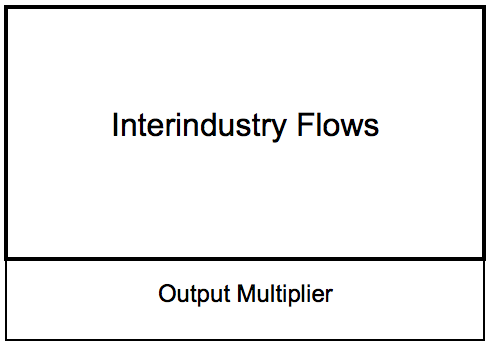
\includegraphics[width=3in]{T1OutputMultiplier}
  \caption{Type I Output Multiplier}
\end{figure}

\bigskip

Below is a brief outline of how the $\textit{A}$-matrix of technical coefficients and the Leontief Inverse is derived. Note that the derivation of the a-coefficients is the same for the different types of multipliers discussed in this section as well as for the types in Section \ref{sec:4.4}.

\bigskip

First, the individual column entries of the inter-industry flows from the IO Tables are divided by the relevant column total. For example, the first sector in the 2009 Scottish IxI Tables is Agriculture \cite{ScottishGovernment2013a}. The figure for the inter-industry flow from Agriculture to Agriculture is \textsterling339m and the column total (``Total output at basic prices'') for Agriculture is \textsterling2,584.3m. This results in the technical coefficient being estimated at 0.131 (this figure corresponds to the $a_{11}$ in Equation \ref{eq:4.3.1}). Note that the $\textit{A}$-matrix below is also labelled as $A_{II}$. The capital i's here are for the industry-by-industry coefficients.

  \bigskip
\begin{singlespacing}
 \begin{equation} \label{eq:4.3.1}
  A = \begin{pmatrix}
  a_{1,1} & \cdots & a_{1,j} \\
  \vdots & \ddots & \vdots  \\
  a_{i,1} & \cdots & a_{i,j}
  \end{pmatrix} \end{equation} 
  \end{singlespacing} \bigskip

The next step in order to be able to calculate the Leontief Inverse, is to construct the $I-\textit{A}$-matrix (see Equation \ref{eq:4.3.4}). This matrix simply uses an identity matrix (see Equation \ref{eq:4.3.2}) and subtracts the $\textit{A}$-matrix (Equation \ref{eq:4.3.1}) from it. The resultant matrix from this calculation has positive values on the diagonal (i.e. the inter-industry flow entries for the individual sectors between themselves). All other entries are negative. Following the example above, the identity matrix gives the value 1 for the Agriculture-Agriculture entry. This is then subtracted by the technical coefficient $a_{11}$  at 0.131. The $(I-A)$-matrix entry (corresponding to $1-a_{11}$ in Equation \ref{eq:4.3.4}) is calculated at 0.869.

  \bigskip \begin{singlespacing} \begin{equation} \label{eq:4.3.2}
  I = \begin{pmatrix}
    1 & \cdots & 0 \\
    \vdots & \ddots & \vdots  \\
    0 & \cdots & 1
  \end{pmatrix} \end{equation} \end{singlespacing} 

  \begin{singlespacing} \begin{equation} \label{eq:4.3.3}
  I-A = \begin{pmatrix}
  1-a_{1,1} & \cdots & 0-a_{1,j} \\
  \vdots & \ddots & \vdots  \\
  0-a_{i,1} & \cdots & 1-a_{i,j}
   \end{pmatrix}   \end{equation} \end{singlespacing}  \bigskip

The last step for the calculation of the Leontief Inverse is inverting the I-A-matrix, thus deriving  $L=(I-A)^{(-1)}$ (see Equation \ref{eq:4.3.4}). The value for the Agriculture-Agriculture entry for the Leontief Inverse is calculated at 1.156 for the Type I output multiplier.

  \bigskip   \begin{singlespacing}  \begin{equation} \label{eq:4.3.4}
  L=(I-A)^{-1} = Inverse  \begin{pmatrix}
    1-a_{1,1} & \cdots & 0-a_{1,j} \\
    \vdots & \ddots & \vdots  \\
    0-a_{i,1} & \cdots & 1-a_{i,j}
  \end{pmatrix}  \end{equation} \end{singlespacing}  \bigskip

The total output multiplier for the Agriculture sector is computed at 1.608 (see Appendix \textcolor{red}A, \ref{sec:4.7.1}).

\subsubsection{Interpretation}

The Type I output multiplier (as outlined above) gives the total value of production for all sectors required to satisfy a \textsterling1m increase in one sector. The Type I provides two distinct output effects. First, the direct effect shows the increase in production needed in sector $i$ to satisfy the initial increase in final demand of \textsterling1m in sector i's output. Second, the indirect effect gives the increase in output that is generated following the direct effect demand response.

\bigskip

For example, if the final demand of the agriculture sector increases by \textsterling1m then the direct effect is a \textsterling1m increase in the Agriculture sector output (to satisfy the increase in final demand). The indirect effect is the additional output response by all other sectors, including the agriculture sector, to the initial shock. This second effect highlights the interdependencies of the various sectors in order to satisfy a final demand increase in one sector.

\subsection{Type II Output Multiplier}
\label{sec:4.3.2}

The Type II output multiplier extends the analysis of the Type I to include households endogenously in the model. The Interindustry flows are supplemented with data on wages and household expenditure. As a result, following a simulated demand shock to the economy, a third effect, the induced effect is also observed.

\subsubsection{Calculation}

The Type II output multiplier allows for a more detailed analysis of a demand shock of the economy due to households being endogenised. Essentially, the household sector is being treated as an additional sector to the model. Figure \ref{fig:4.3.2}visualizes the addition to the multiplier calculation. In comparison to Figure \ref{fig:4.3.1} (see Section \ref{sec:4.3.1}), the data on the interindustry flows are supplemented by data on wages (Income from Employment row) and data on household expenditure (Households column) in Figure \ref{fig:4.3.2}. Note, however, that the calculated entries of the Leontief Inverse matrix for the Income from Employment row are not added to the sum for the output multiplier. Adding the entries of the Income from Employment row results in the Gross Value Added (GVA) multiplier. According to \citeA[p.248]{Miller2009} the Type II shown in Appendix \textcolor{red}A, \ref{sec:4.7.1} are the truncated output multiplier.

\bigskip
\begin{figure}[hb]
\label{fig:4.3.2}
  \centering
  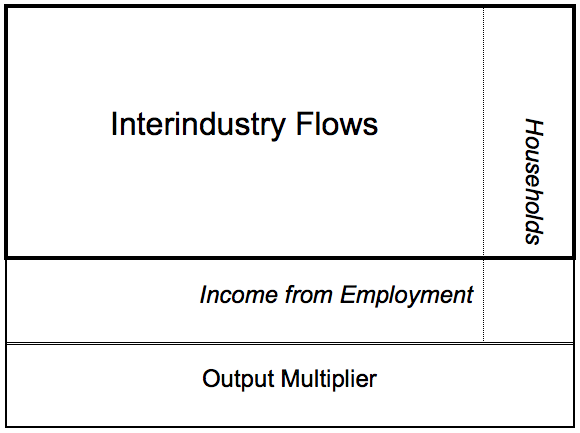
\includegraphics[width=3.5in]{T2OutputMultiplier}
  \caption{Type I Output Multiplier}
\end{figure}
\bigskip

The data used for the additional (Income from Employment) row for the Type II output multiplier (see Figure \ref{fig:4.3.2}), are wages. The IxI Tables give the ``Compensation of Employees'' for wages received. The corresponding total by which this row is divided in order to derive the $\textit{A}$-matrix entry for the Income from Employment row is the same as for the Interindustry flows. That is each sector's column total, the ``Total Output at basic prices''.

\bigskip

The second part for endogenising the Household sector is shown as the Households column in  Figure \ref{fig:4.3.2}. The cells used for this from the IxI Tables are the Household sectors ``Final Consumption Expenditure''. Note that this data is used in all the methods discussed in  Section \ref{sec:4.4}. The total used for the division of the Household cells for the A-matrix differs, however. Assessing which of these totals provides the best fit in comparison with the SAM multiplier is the motivation of this paper. For the purpose of illustration this paper uses the total from the Miller and Blair \citeA{Miller2009} method (see Section \ref{sec:4.4.1}). The total here for deriving the $a$-coefficients for the Household sector is the  ``Total Intermediate Demand'' of the ``Compensation of employees'' row at \textsterling63,560.9m \cite{ScottishGovernment2013a}.

\bigskip

Following the computation of the matrix of technical coefficients outlined above, the Leontief Inverse is computed. The method here is the same as for the Type I output multiplier in Section \ref{sec:4.3.1} (Equation \ref{eq:4.3.2} to \ref{eq:4.3.4}). The Leontief Inverse for the Type II is shown in Equation \ref{eq:4.3.5}.

  \bigskip  \begin{singlespacing}  \begin{equation} \label{eq:4.3.5}
  L=(I-A)^{-1} = Inverse   \begin{pmatrix}
  A_{II} &  A_{IH} \\
  A_{HI}  & A_{HH}
  \end{pmatrix} 
  \end{equation}   \end{singlespacing}  \bigskip

Equation \ref{eq:4.3.5} shows that the Leontief Inverse for the Type II multiplier now consists of additional technical coefficient entries in contrast to Equation \ref{eq:4.3.4}. These additions reflect the endogenised Household sector. $A_{II}$ is the technical coefficient matrix for the interindustry flows equal to Equation \ref{eq:4.3.1}. $A_{IH}$ is the amount of industry output required to satisfy Household demand. $A_{HI}$ is the amount of industry required per unit of total household income. $A_{HH}$ is household expenditure per unit of exogenous household income \cite{ScottishGovernment2013a}.

\bigskip

The computed value for the Agriculture-Agriculture entry for the Leontief Inverse differs to that of the Type I (see Section \ref{sec:4.3.1}). The Type I value is 1.156 and that for the Type II is 1.163 \footnote{ Note that this value differs depending on which method of the Type II output multiplier is used (see Section \ref{sec:4.3.1}).}. The Type II output multiplier is also bigger, as it is now 1.963, compared to 1.608 for the Type I. The following Section discusses the increase in multiplier value from Type I to Type II.

\subsubsection{Interpretation}

As noted above, the Type II output multiplier \footnote{ The Miller and Blair \citeA{Miller2009} method is used here for illustrative purposes (see Section \ref{sec:4.4.1}).} is larger than that of the Type I. This is due to the fact that the Type II multiplier models both the direct and indirect effects (like the Type I) as well as the induced effect. The induced effect results from the endogenising of the Household sector, as outlined in the Section above (see Section \ref{sec:4.3.2}).

\bigskip

Section \ref{sec:4.3.2})above outlined the direct effect and the indirect effect a demand shock of \textsterling1m in one sector. The induced effect observed in the Type II output multiplier results from additional household expenditure. The demand shock results in an output response throughout the economy (the direct- and indirect effects). It is assumed that the increase in output also has a positive effect on wages. Due to higher wages the Household sector increases expenditure and this is the induced effect.

\bigskip

Comparing the value of a Type I and a Type II output multiplier allows for the observation of the size of the induced effect. Following on from the example above, the Type II output multiplier (using the Miller and Blair \citeA{Miller2009} method introduced in Section \ref{sec:4.4.1}) below) is bigger by 0.355 \footnote{ The Type I output multiplier for Agriculture is computed at 1.608 and the Miller and Blair \citeA{Miller2009} Type II one at 1.963.}. Thus the initial \textsterling1m demand shock results in a multiplier effect in household expenditure of \textsterling355,000. Note that the size of the induced effect differs depending on which method of the Type II output multiplier is used.

\subsection{SAM Output Mulltiplier}
\label{sec:4.3.3}

The SAM output multiplier offers the most inclusive study of the multipliers discussed in this Section. As well as endogenising the Household sector, the SAM output multiplier also endogenises the Corporate sector. It uses a more comprehensive dataset and thus relies on more assumptions than the Type I or Type II output multiplier. Also note that the SAM output multiplier can only be computed in the presence of a suitable SAM.

\subsubsection{Calculation}

The basic calculation of the SAM output multiplier is very similar to the one outlined for the Type II in the Section above (see Section \ref{sec:4.3.2}). Figure \ref{fig:4.3.3}) shows which elements need to be added to the computation of the SAM output multiplier in order to endogenise the Corporate sector as well as the Household sector.

\bigskip
\begin{figure}[hb]
\label{fig:4.3.3}
  \centering
  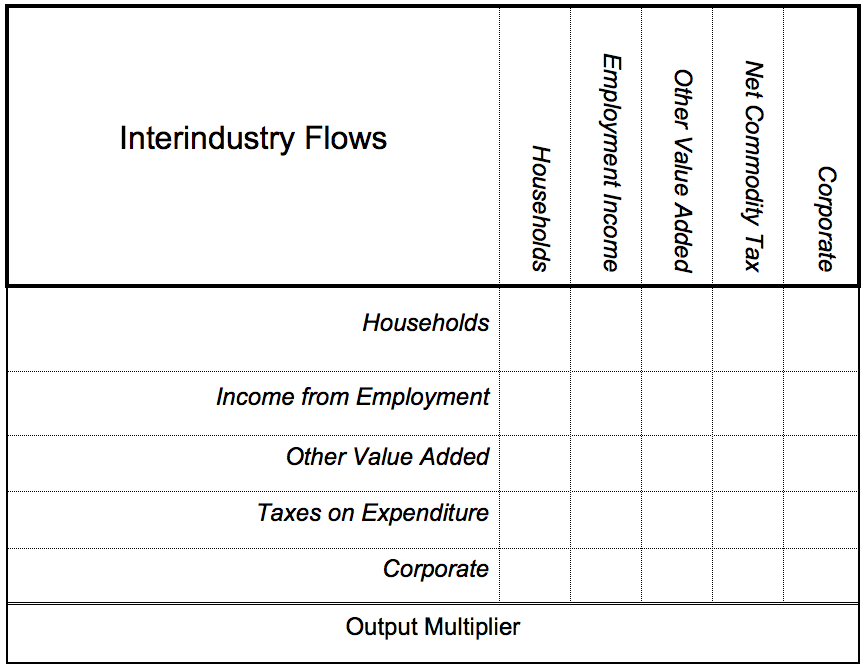
\includegraphics[width=4.5in]{SAMOutputMultiplier}
  \caption{Type I Output Multiplier}
\end{figure}
\bigskip

Equation \ref{eq:4.3.6} shows the Leontief Inverse of the SAM output multiplier. The interindustry matrix of technical coefficients is the $A_{II}$ in Equation \ref{eq:4.3.6}. The other data used for endogenising the Corporate Sector as well as the Household sector are shown as the additional row and column entries in Equation \ref{eq:4.3.6}. The interpretation of these vectors is equivalent to the added entries in Equation \ref{eq:4.3.5} (see Section \ref{sec:4.3.2}).

  \bigskip \begin{singlespacing}  \begin{equation} \label{eq:4.3.6}
  L=(I-A)^{-1} = Inverse   \begin{pmatrix}
  A_{II} & \cdots & A_{IC}  \\
  \vdots & \ddots & \vdots  \\
  A_{CI} & \cdots & A_{CC}
  \end{pmatrix} \end{equation} \end{singlespacing}  \bigskip

Note that the rows shown below the interindustry flows in Figure \ref{fig:4.3.3} are also not added to the multiplier figure (see Section \ref{sec:4.3.2} for comparison).

\subsubsection{Interpretation}

The interpretation of the SAM output multiplier follows along that of the Type II in Section \ref{sec:4.3.2}. The SAM multiplier computed here treats the Household- and the Corporate sector as endogenous.

\bigskip

... more

\bigskip

%%%%%%%%%%%%%%%%%%%%%%%%%%%%%%%%%%%%%%%%%%%%%%%%%%%%%%%%%%
%SECTION
%%%%%%%%%%%%%%%%%%%%%%%%%%%%%%%%%%%%%%%%%%%%%%%%%%%%%%%%%%

\newpage
    \section{Four Type II Methods}
\label{sec:4.4}

The previous Section outlined how the Type I, the Type II and the SAM output multiplier are computed. This basic structure for the derivation of these multipliers is used throughout the literature \textcolor{red}{REF} \footnote{ Additionally, there are various extensions for the Type II multiplier in particular \textcolor{red}{REF}, but this paper is concerned with the standard derivation of the Type II output multiplier.}. However, there are variations in what totals should be used for endogenising the Household sector in the Type II output multiplier as outlined in Section \ref{sec4.3.2}.

\bigskip

This Section outlines four methods used for the computation of the Type II output multiplier for Scotland. Section 5 analyses the results and compares the multipliers with each other. A benchmark value is needed in order to compare the different Type II multiplier methods. For this, it is assumed that the most complete set of accounts for the flow of goods and services in Scotland are given in a 2009 SAM for Scotland \cite{SCOSAM}. Thus, the SAM output multiplier is calculated and used as a benchmark \footnote{Note that a SAM multiplier automatically includes the Income from Employment and Household coefficients and thus is suitable to be used for a benchmark of the IO Type II's.}. The inter-industry flows as well as the Income from Employment and Household entries are the same for the IO and the SAM multiplier calculations. The variation of the multiplier values for the methods outlined below is due in part to the different Totals used for endogenising the Household sector. Thus the assumption is that the Totals closest in value to the Total used in the SAM multiplier calculations will derive the closest fitting multipliers.

\subsection{Miller and Blair}
\label{sec:4.4.1}

The first method analysed here originates from \citeA{Miller2009}, who use the total of the ``Compensation of Employee'' as the denominator for the technical coefficients of the Household sector \footnote{ Note, that this is the total of the Income from Employment row used by all four approaches.}. The corresponding value of this entry in the 2009 Scottish IxI Table is \textsterling63,561m \cite{ScottishGovernment2013a}.

\subsection{IxI Household Expenditure Total}
\label{sec:4.4.2}

The second method uses the ``Total Intermediate Consumption at basic prices'' of ``Households’ Final Consumption Expenditure''. This value is also given in the IxI Table and amounts to \textsterling65,421m \cite{ScottishGovernment2013a}.

\subsection{SAM Output Mulltiplier}
\label{sec:4.4.3}

The third method uses the total expenditure of the Household sector from the 2009 Scottish SAM \cite{SCOSAM}. This figure is derived by first, summing up the ``Final Consumption Expenditure'' of Households and ``Final Consumption Expenditure'' of Non-Profit Organisations Serving Households (NPISHs). Second, the Household expenditure on goods \& services of the following sectors are added to the Household Total: Rest of The World, Rest of the UK, Corporate, Government and Capital. This figure amounts to \textsterling107,877m.

\subsection{SAM Output Multiplier}
\label{sec:4.4.4}

The fourth method uses the combined Compensation of Employees at \textsterling63,561m from the IxI Table \footnote{ This is the Total used in the \citeA{Miller2009} method.} \cite{ScottishGovernment2013a} and all Unearned Income at \textsterling46,835m \cite{ScotGov2013c}. The total here is \textsterling110,396m. This figure is similar in nature to the one taken from the SAM above as it incorporates additional Household income sources. This is in contrast to the pure wage figures used, for example, in the \citeA{Miller2009} method. It is also the figure used for the official Scottish Government Leontief Inverse calculations.

\bigskip

Following on from the assumption placed above, the method using the Scottish SAM Household Total for endogenising the Household sector ought to be closest to the values derived by the SAM output multiplier. That is, the SAM uses the same Household Total for endogenising the Household sector. Next, the Combined Household Income Total is expected be closest. Then in descending order from Household Total value, the IxI Household Expenditure Total should give the third closest Type II estimate and lastly the one derived through the \citeA{Miller2009} method. However, it is worth noting that the Scottish SAM Household Total can only be used to derive the (IO) Type II if there is an applicable SAM. Hence the question arises whether pure IO modelling would allow for the presence of this type of IO multiplier.

%%%%%%%%%%%%%%%%%%%%%%%%%%%%%%%%%%%%%%%%%%%%%%%%%%%%%%%%%%
%SECTION
%%%%%%%%%%%%%%%%%%%%%%%%%%%%%%%%%%%%%%%%%%%%%%%%%%%%%%%%%%



%%%%%%%%%%%%%%%%%%%%%%%%%%%%%%%%%%%%%%%%%%%%%%%%%%%%%%%%%%%%%%%%%%%%%%%%%%%%%%%%%%%%%%%%%%%%%%%%%%%%%%%%%%%%%%%%%%%%%%%%%%%%%%%% SECTION 5
%%%%%%%%%%%%%%%%%%%%%%%%%%%%%%%%%%%%%%%%%%%%%%%%%%%%%%%%%%%%%%%%%%%%%%%%%%%%%%%%%%%%%%%%%%%%%%%%%%%%%%%%%%%%%%%%%%%%%%%%%%%%%%%%

\newpage
    \section{Results}
\label{sec:4.5}

This Section discusses the results of the multiplier computations. First, the raw multiplier values are discussed using descriptive analysis. Second, the different Type II output multipliers are compared to the SAM output multiplier using difference statistics. Third, error computations are utilized to determine a best fit of one of the four Type II output multipliers compared to the SAM output multiplier. Fourth, the results are summarized to provide a comprehensive overview of the findings in this Section.

\subsection{Multiplier Descriptives}
\label{sec:4.5.1}

Appendix A provides a full breakdown of the Type I, the Type II and the SAM output multipliers derived for 102 sectors of the 2009 Scottish IxI Tables and the 2009 Scottish SAM. This table allows for an in-depth analysis of the value of each multiplier for each sector. 

\bigskip

Furthermore, Appendix A shows the average values for each type of output multiplier. The Type I output multiplier is the lowest on average. This is to be expected, since this multiplier is computed using only the interindustry flow data from the IxI Tables. In contrast, the two largest average multiplier values are derived using the Miller and Blair and the IxI Household Expenditure Total methods (see Sections \ref{sec:4.4.1} and \ref{sec:4.4.2} ). Again this is to be expected, because these two methods use smaller values for the endogenising of the Household sector \footnote{The Miller and Blair value is \textsterling63,561m, and the IxI Household Expenditure Total value is \textsterling65,421m.}. In comparison, the other two methods outlined in Section \ref{sec:4.4} (see Sections \ref{sec:4.4.3} and \ref{sec:4.4.4}) use higher values for the endogenising of the Household sector \footnote{The Scottish SAM Household Total value is \textsterling107,877m, the Combined Household Income Total value is \textsterling110,396m.}. 

\bigskip

Using the SAM output multiplier as a benchmark, the average values show that the Miller and Blair as well as the IxI Household Expenditure Total method overestimate the average output multiplier effect. In contrast, the Scottish SAM Household Total and the Combined Household Income Total method underestimate the average output multiplier effect. Note though that the average difference of the latter compared to the SAM output multiplier is smaller. Lastly, Appendix A also shows the minimum and maximum multiplier values. These values reflect the analytics from above.


\bigskip
\begin{centering}
  \begin{table}[H]
\centering
  \caption{Descriptives Output Multiplier}
  \bigskip \begin{scriptsize}  \begin{doublespacing}
  \begin{tabular}{lrrrrrr}
  \toprule
   &  \begin{sideways}Type I\end{sideways} & \begin{sideways}Miller and Blair\end{sideways} & \begin{sideways}Scot Gov Stev\end{sideways} & \begin{sideways}Scot Gov SAM\end{sideways} & \begin{sideways}HH Exp\end{sideways} & \begin{sideways}SAM\end{sideways}   \bigstrut[b]\\
  \hline
           Average & 1.465 & 2.096 & 1.778 & 1.787 & 2.072 & 1.910 \\
           Minimum & 1.000 & 1.214 & 1.182 & 1.183 & 1.212 & 1.321 \\
           Maximum & 2.780 & 3.295 & 3.035 & 3.042 & 3.275 & 3.214 \\
  \hline \hline
      \end{tabular}%
        \bigskip  \label{tab:4.5.1}
      \end{doublespacing}  \end{scriptsize} \end{table}
      \end{centering}
\bigskip

\subsection{Multiplier Difference Statistics}
\label{sec:4.5.2}

Appendix B shows the differences between the Type II multiplier methods and the SAM benchmark. This allows for an in-depth study of which method of the multiplier is closest in value to the SAM multiplier broken down by individual sectors. This detailed analysis shows that there is not one method, which is closest in value for all sectors. For example, the first sector Agriculture shows that the Miller and Blair \cite{Miller2009} method gives the closest fitting multiplier at a value of 0.001\footnote{This value is calculated by taking the SAM multiplier value for the Agriculture sector of 1.964 and subtracting it by the relevant Miller and Blair method multiplier, which has a value of 1.963.}. For the same sector, the multiplier figure from the Combined Household Income Total shows the biggest difference at 0.180. In comparison, looking at the last sector, Households as Employers, using the SAM Household Income figure shows the smallest difference at 0.145. Here, the Miller and Blair \cite{Miller2009} version gives the biggest gap compared to the SAM at -0.485 with the Household Expenditure method following close behind at -0.435. This detailed analysis offers insights into which method might be offer the closest fit for different sectors. 

\bigskip

Note that the first two methods (Miller and Blair; IxI Household Expenditure Total) have mostly negative differences to the benchmark (see Appendix B)\footnote{Whilst the majority of sectors follow the same pattern, there are five sectors that diverge. Large differences between OVA and wages in those sectors seem to cause the reversed signs.}. In contrast, the last two methods described above (Scottish SAM Household Total; Combined Household Income Total) show only positive differences. These findings seem to suggest that the first two methods overestimate the Leontief Inverse. In contrast, the last two methods underestimate the Leontief Inverse compared to the benchmark. In order to be able to analyse which methods are closer to the benchmark, the absolute values of the differences in Appendix B are calculated (Appendix C).

\bigskip

The graph in Appendix C gives the ``Absolute Value Difference''\footnote{Absolute Value Differences - see word file}. The horizontal axis here can be interpreted to represent the SAM multiplier value and thus the closer the lines are to this axis, the better the fit. This graph shows that the two Type II methods using the more comprehensive household figure, the Scottish SAM Household Total and the Combined Household Income Total, give the closest fit to the SAM multiplier. The graph also strongly depicts that these two methods vary less in value compared to the first two Type II methods discussed above. The Miller and Blair \cite{Miller2009} method shows the overall biggest differences to the benchmark. In contrast, the Scottish SAM Household Total provides the closest fit in the graph. This confirms that endogenising the household sector using the SAM Household Total results in the closest fit.

\bigskip

Furthermore, Appendix C highlights that the difference between the methods varies substantially between the sectors. The methods using the Scottish SAM Household Total and the Combined Household Income Total for endogenising the Household sector show some variation compared to the benchmark. However, there are some very pronounced spikes observable in Appendix C for the Miller and Blair and the IxI Household Expenditure Total methods. The three biggest differences are for the Education (93), Security \& Investigation (89) and the Social Work (96) sectors. The multipliers for these sectors show large variation in comparison to the SAM output multiplier. These differences seem to be due to a small Gross Value Added to Total Output gap in the IxI Tables (REF).


\subsection{Error Computation}
\label{sec:4.5.3}

Table 1 shows various error-computations of the methods outlined above and the SAM benchmark. This allows for detailed measurements of the differences between the methods. The error-measurements in Table 1 are the ``Average of Differences''\footnote{This is the average of the differences for each sectoral multiplier derived from Appendix B.}, the Root Mean Squared Error (RMSE) and the Mean Absolute Error (MAE). The smallest value indicates the best fit with respect to the SAM output multiplier. All measurements show that endogenising the Household sector using the Scottish SAM Household Total figure results in the closest fit, followed by using the Combined Household Income Total figure. These two methods do not differ much in the error values. Also note that the values in Table 1 show that the four methods can be classified into two groups. First, the methods using pure IO data and second, the methods using the more comprehensive household expenditure figures. An example is the ``Average of Difference'' for Miller and Blair and the Household Expenditure total are estimated at 0.186 and 0.161, respectively. The same error computation for the Household Income from the SAM is given at 0.124 and that for the Household Income Scottish Government at 0.132.


\bigskip
\begin{centering}
  \begin{table}[H]
\centering
  \caption{RMSE and MAE Errors}
  \bigskip \begin{scriptsize}  \begin{doublespacing}
  \begin{tabular}{lrrrr}
  \toprule
  &  \begin{sideways}Miller and Blair\end{sideways} & \begin{sideways}Scot Gov Stev\end{sideways} & \begin{sideways}Scot Gov SAM\end{sideways} & \begin{sideways}HH Exp\end{sideways}   \bigstrut[b]\\
  \hline
  Average of Differences &  0.186 & 0.161 & 0.124 & 0.132   \\
  RMSE & 0.156 & 0.138 & 0.093 & 0.099   \\
  MAE & 0.101 & 0.089 & 0.065 & 0.070    \bigstrut[b]\\
  \hline \hline
  \multicolumn{5}{l}{Note: Smallest value shows closest fit to SAM multipliers}
      \end{tabular}%
        \bigskip  \label{tab:4.5.2}
      \end{doublespacing}  \end{scriptsize} \end{table}
      \end{centering}
\bigskip


The values in Table 1 also confirm that the Miller and Blair method results in the least close fit compared to the benchmark. In comparison, endogenising household expenditure using the IxI Household expenditure total, the Household sector column Total (2nd method from the left in Table 1) results in a closer fit. For example, the RMSE for the Miller and Blair method is given at 0.156 and the RMSE for the Household Expenditure total at 0.138. Therefore these results seem to suggest that computing a Type II with figures given only in the IO Tables would result in more accurate computations using the Household Expenditure total. 

\bigskip

The overall smallest error values are computed using the Scottish SAM Household Total. For example, is the MAE for this method is 0.065 and the next closest fit, the Combined Household Income Total, is 0.070. As noted above, the benchmark here is the SAM multiplier, due to the assumption that the 2009 Scottish SAM provides the most comprehensive single set of accounts of the Scottish economy for 2009. However, it is questionable whether pure IO modeling allows for the use of the SAM Household figure in endogenising household expenditure.

\subsection{Summary of Results}
\label{sec:4.5.4}

The general finding of this paper is that using more comprehensive household expenditure totals result in the closest fit of the Type IIs in comparison to the output multiplier derived from IxI data. An explanation for this is that not all household expenditure is covered using the income from employment figures from the Miller and Blair as well as the IxI Household Expenditure Total from the IxI Tables. Unearned income is part of households’ budgets and thus households’ total funds are bigger than those provided just in the IO Tables. Using these smaller income figures (Miller and Blair and IxI Household Expenditure Total) for endogenising household expenditure for the multiplier analysis is assumed to result in an overestimated Leontief Inverse. This in turn leads to a larger induced effect than is actually observed in the economy (REF IO Guide).

\bigskip

The findings in Appendix C confirm that using the first two methods result in overestimated figures of the Leontief Inverse. It must be noted, however, that the two methods using the more comprehensive Household Totals result in underestimated Leontief Inverses compared to the benchmark. Yet, the latter two methods observe smaller differences compared to the benchmark. 


%%%%%%%%%%%%%%%%%%%%%%%%%%%%%%%%%%%%%%%%%%%%%%%%%%%%%%%%%%%%%%%%%%%%%%%%%%%%%%%%%%%%%%%%%%%%%%%%%%%%%%%%%%%%%%%%%%%%%%%%%%%%%%%% SECTION 6
%%%%%%%%%%%%%%%%%%%%%%%%%%%%%%%%%%%%%%%%%%%%%%%%%%%%%%%%%%%%%%%%%%%%%%%%%%%%%%%%%%%%%%%%%%%%%%%%%%%%%%%%%%%%%%%%%%%%%%%%%%%%%%%%

\newpage
    \section{Conclusion}
\label{sec:4.6}

This paper shows that using the Total Household Income figure from the SAM for endogenising the Household sector results in the best multiplier fit. Note though that some of the other multiplier methods discussed above show closer fits for individual sectors. The overall best fit of the SAM Household Total method is to be expected since the SAM output multiplier is used as the benchmark. It is questionable, however, whether using a SAM entry for the derivation of an IO multiplier is theoretically correct. Similarly, using the Combined Household Income Total value for endogenising the Household sector relies on the availability of a data source exogenous to the IxI Tables. This paper finds that using the IxI Total Household Expenditure Total method is the best fit if the methods using exogenous data to the IxI Tables are not used. Thus, this paper has also shown that the widely used Miller and Blair method (REF) often derives the least best fitting Type II output multipliers. Thus, using the IxI Total Household Expenditure Total figure for the derivation of a pure IO Type II results in more accurate multipliers overall. 

\end{doublespacing}

\newpage
    \section{Appendix}
\label{sec:4.7}

\subsection{Appendix A}
\label{sec:4.7.1}
\bigskip
\textbf{Output Multiplier}

\begin{longtable}{@{\extracolsep{\fill}}rlrrrrrr@{}}
  &&  \begin{sideways}Type I\end{sideways} & \begin{sideways}Miller and Blair\end{sideways} & \begin{sideways}Scot Gov Stev\end{sideways} & \begin{sideways}Scot Gov SAM\end{sideways} & \begin{sideways}HH Exp\end{sideways} & \begin{sideways}SAM\end{sideways} \\ [0.5ex] 
    \hline 
    1     & Agriculture & 1.608 & 1.963 & 1.784 & 1.789 & 1.949 & 1.964 \\
    2     & Forestry planting & 1.615 & 2.069 & 1.840 & 1.846 & 2.051 & 1.972 \\
    3     & Forestry harvesting & 1.961 & 2.469 & 2.213 & 2.220 & 2.449 & 2.367 \\
    4     & Fishing & 1.611 & 1.962 & 1.785 & 1.790 & 1.949 & 1.933 \\
    5     & Aquaculture & 1.625 & 1.928 & 1.775 & 1.779 & 1.916 & 1.916 \\
    6     & Coal \& lignite & 1.671 & 2.079 & 1.874 & 1.879 & 2.063 & 1.983 \\
    8     & Other mining & 1.435 & 1.938 & 1.684 & 1.691 & 1.918 & 1.786 \\
    9     & Mining Support & 1.501 & 1.827 & 1.663 & 1.667 & 1.815 & 1.847 \\
    10    & Meat processing & 1.917 & 2.367 & 2.141 & 2.147 & 2.350 & 2.250 \\
    11    & Fish \& fruit processing & 1.695 & 2.184 & 1.937 & 1.944 & 2.165 & 2.044 \\
    12    & Dairy prod., oils \& fats processing & 1.923 & 2.430 & 2.174 & 2.181 & 2.410 & 2.300 \\
    13    & Grain milling \& starch & 1.803 & 2.257 & 2.028 & 2.035 & 2.240 & 2.134 \\
    14    & Bakery \& farinaceous & 1.426 & 2.031 & 1.726 & 1.735 & 2.007 & 1.840 \\
    15    & Other food & 1.609 & 2.139 & 1.872 & 1.879 & 2.118 & 1.980 \\
    16    & Animal feeds & 1.589 & 2.043 & 1.814 & 1.820 & 2.026 & 1.897 \\
    17    & Spirits \& wines & 1.299 & 1.738 & 1.516 & 1.523 & 1.721 & 1.694 \\
    18    & Beer \& malt & 1.367 & 1.775 & 1.570 & 1.575 & 1.760 & 1.746 \\
    19    & Soft Drinks & 1.493 & 2.009 & 1.749 & 1.756 & 1.989 & 1.872 \\
    21    & Textiles & 1.436 & 2.052 & 1.742 & 1.750 & 2.028 & 1.830 \\
    22    & Wearing apparel & 1.465 & 2.174 & 1.817 & 1.826 & 2.147 & 1.907 \\
    23    & Leather goods & 1.497 & 2.082 & 1.787 & 1.795 & 2.060 & 1.890 \\
    24    & Wood and wood products & 1.801 & 2.423 & 2.109 & 2.118 & 2.399 & 2.223 \\
    25    & Paper \& paper products & 1.662 & 2.163 & 1.911 & 1.918 & 2.144 & 2.010 \\
    26    & Printing and recording & 1.378 & 2.159 & 1.766 & 1.776 & 2.129 & 1.883 \\
    27    & Coke, petroleum \& petrochemicals & 1.204 & 1.302 & 1.253 & 1.254 & 1.299 & 1.321 \\
    28    & Paints, varnishes and inks etc & 1.421 & 1.924 & 1.671 & 1.678 & 1.905 & 1.756 \\
    29    & Cleaning \& toilet preparations & 1.460 & 2.139 & 1.797 & 1.806 & 2.113 & 1.895 \\
    30    & Other chemicals & 1.251 & 2.026 & 1.635 & 1.646 & 1.996 & 1.765 \\
    31    & Inorg. chem., dyestuffs \& agrochem. & 1.314 & 1.886 & 1.597 & 1.605 & 1.863 & 1.716 \\
    32    & Pharmaceuticals & 1.349 & 1.961 & 1.652 & 1.661 & 1.937 & 1.776 \\
    33    & Rubber \& Plastic & 1.491 & 2.199 & 1.843 & 1.852 & 2.172 & 1.948 \\
    34    & Cement lime \& plaster & 1.594 & 2.200 & 1.895 & 1.903 & 2.177 & 1.997 \\
    35    & Glass, clay \& stone etc & 1.473 & 2.144 & 1.806 & 1.815 & 2.118 & 1.915 \\
    36    & Iron \& Steel & 1.401 & 2.010 & 1.703 & 1.712 & 1.987 & 1.803 \\
    37    & Other metals \& casting & 1.449 & 1.982 & 1.713 & 1.721 & 1.962 & 1.831 \\
    38    & Fabricated metal & 1.481 & 2.185 & 1.830 & 1.840 & 2.157 & 1.941 \\
    39    & Computers, electronics \& opticals & 1.416 & 1.931 & 1.671 & 1.679 & 1.911 & 1.767 \\
    40    & Electrical equipment & 1.483 & 2.123 & 1.800 & 1.809 & 2.098 & 1.896 \\
    41    & Machinery \& equipment & 1.519 & 2.236 & 1.875 & 1.885 & 2.209 & 1.983 \\
    42    & Motor Vehicles & 1.515 & 2.121 & 1.816 & 1.824 & 2.098 & 1.907 \\
    43    & Other transport equipment & 1.647 & 2.211 & 1.927 & 1.935 & 2.190 & 2.026 \\
    44    & Furniture & 1.574 & 2.223 & 1.896 & 1.905 & 2.198 & 1.999 \\
    45    & Other manufacturing & 1.403 & 2.224 & 1.811 & 1.822 & 2.193 & 1.913 \\
    46    & Repair \& maintenance & 1.427 & 2.101 & 1.761 & 1.770 & 2.074 & 1.877 \\
    47    & Electricity & 2.053 & 2.375 & 2.213 & 2.217 & 2.363 & 2.345 \\
    48    & Gas etc & 1.260 & 1.519 & 1.389 & 1.392 & 1.509 & 1.482 \\
    49    & Water and sewerage & 1.287 & 1.694 & 1.489 & 1.495 & 1.679 & 1.708 \\
    50    & Waste & 1.493 & 2.135 & 1.811 & 1.820 & 2.110 & 1.941 \\
    51    & Remediation \& waste managem. & 2.780 & 3.295 & 3.035 & 3.042 & 3.275 & 3.214 \\
    52    & Construction - buildings & 1.766 & 2.347 & 2.054 & 2.062 & 2.324 & 2.200 \\
    53    & Construction - civil engineering & 1.731 & 2.388 & 2.057 & 2.066 & 2.363 & 2.202 \\
    54    & Construction - specialised & 1.530 & 2.223 & 1.874 & 1.883 & 2.196 & 2.020 \\
    55    & Wholesale \& Retail - vehicles & 1.335 & 2.049 & 1.689 & 1.699 & 2.021 & 1.815 \\
    56    & Wholesale - excl vehicles & 1.521 & 2.190 & 1.853 & 1.862 & 2.164 & 1.990 \\
    57    & Retail - excl vehicles & 1.352 & 2.071 & 1.709 & 1.719 & 2.044 & 1.858 \\
    58    & Rail transport & 1.764 & 2.512 & 2.135 & 2.145 & 2.483 & 2.265 \\
    59    & Other land transport & 1.400 & 1.979 & 1.687 & 1.695 & 1.956 & 1.810 \\
    60    & Water transport & 1.657 & 2.097 & 1.875 & 1.881 & 2.080 & 1.980 \\
    61    & Air transport & 1.467 & 1.881 & 1.672 & 1.678 & 1.865 & 1.792 \\
    62    & Support services for transport & 1.541 & 2.139 & 1.838 & 1.846 & 2.116 & 1.994 \\
    63    & Post \& courier & 1.278 & 2.259 & 1.765 & 1.778 & 2.221 & 1.893 \\
    64    & Accommodation & 1.352 & 2.004 & 1.675 & 1.684 & 1.979 & 1.814 \\
    65    & Food \& beverage services & 1.362 & 2.020 & 1.688 & 1.697 & 1.995 & 1.816 \\
    66    & Publishing services & 1.279 & 2.066 & 1.670 & 1.681 & 2.036 & 1.790 \\
    67    & Film video \& TV etc & 1.454 & 2.045 & 1.747 & 1.755 & 2.022 & 1.869 \\
    68    & Broadcasting & 1.386 & 1.987 & 1.684 & 1.692 & 1.963 & 1.819 \\
    69    & Telecommunications & 1.393 & 2.009 & 1.699 & 1.707 & 1.985 & 1.859 \\
    70    & Computer services & 1.250 & 2.041 & 1.642 & 1.653 & 2.010 & 1.789 \\
    71    & Information services & 1.185 & 1.918 & 1.549 & 1.559 & 1.890 & 1.719 \\
    72    & Financial services & 1.222 & 1.736 & 1.477 & 1.484 & 1.716 & 1.665 \\
    73    & Insurance \& pensions & 1.859 & 2.316 & 2.086 & 2.092 & 2.298 & 2.234 \\
    74    & Auxiliary financial services & 1.282 & 2.065 & 1.670 & 1.681 & 2.035 & 1.796 \\
    75    & Real estate - own & 1.465 & 1.742 & 1.603 & 1.606 & 1.732 & 1.817 \\
    76    & Imputed rent & 1.151 & 1.214 & 1.182 & 1.183 & 1.212 & 1.387 \\
    77    & Real estate - fee or contract & 1.503 & 2.139 & 1.818 & 1.827 & 2.114 & 1.971 \\
    78    & Legal activities & 1.241 & 1.998 & 1.617 & 1.627 & 1.969 & 1.781 \\
    79    & Accounting \& tax services & 1.202 & 2.040 & 1.617 & 1.629 & 2.007 & 1.786 \\
    80    & Head office \& consulting services & 1.391 & 2.192 & 1.789 & 1.800 & 2.161 & 1.914 \\
    81    & Architectural services etc & 1.437 & 2.171 & 1.801 & 1.811 & 2.142 & 1.953 \\
    82    & Research \& development & 1.423 & 2.439 & 1.927 & 1.941 & 2.400 & 2.057 \\
    83    & Advertising \& market research & 1.250 & 1.953 & 1.599 & 1.608 & 1.926 & 1.772 \\
    84    & Other professional services & 1.330 & 1.978 & 1.651 & 1.660 & 1.953 & 1.801 \\
    85    & Veterinary services & 1.364 & 2.126 & 1.742 & 1.752 & 2.096 & 1.918 \\
    86    & Rental and leasing services & 1.324 & 1.861 & 1.590 & 1.598 & 1.840 & 1.751 \\
    87    & Employment services & 1.301 & 2.261 & 1.778 & 1.791 & 2.224 & 1.918 \\
    88    & Travel \& related services & 1.520 & 1.900 & 1.709 & 1.714 & 1.886 & 1.786 \\
    89    & Security \& investigation & 1.155 & 2.273 & 1.709 & 1.725 & 2.229 & 1.853 \\
    90    & Building \& landscape services & 1.388 & 2.248 & 1.815 & 1.826 & 2.215 & 1.964 \\
    91    & Business support services & 1.285 & 1.925 & 1.602 & 1.611 & 1.900 & 1.769 \\
    92    & Public administration \& defence & 1.410 & 2.169 & 1.786 & 1.797 & 2.139 & 1.903 \\
    93    & Education & 1.189 & 2.367 & 1.774 & 1.790 & 2.322 & 1.914 \\
    94    & Health & 1.362 & 2.210 & 1.782 & 1.794 & 2.177 & 1.902 \\
    95    & Residential care & 1.320 & 2.243 & 1.778 & 1.791 & 2.207 & 1.950 \\
    96    & Social work & 1.236 & 2.388 & 1.807 & 1.823 & 2.343 & 1.959 \\
    97    & Creative services & 1.474 & 2.319 & 1.893 & 1.905 & 2.286 & 2.005 \\
    98    & Cultural services & 1.356 & 2.294 & 1.821 & 1.834 & 2.258 & 1.948 \\
    99    & Gambling & 1.414 & 1.888 & 1.649 & 1.656 & 1.870 & 1.822 \\
    100   & Sports \& recreation & 1.407 & 2.253 & 1.826 & 1.838 & 2.220 & 1.950 \\
    101   & Membership organisations & 1.436 & 2.253 & 1.841 & 1.852 & 2.221 & 1.970 \\
    102   & Repairs - personal and household & 1.357 & 2.055 & 1.703 & 1.713 & 2.028 & 1.822 \\
    103   & Other personal services & 1.233 & 1.886 & 1.557 & 1.566 & 1.861 & 1.732 \\
    104   & Households as employers & 1.000 & 2.284 & 1.637 & 1.655 & 2.234 & 1.799 \\
\hline
\caption{Output Multiplier}
\end{longtable}

\newpage

\subsection{Appendix B}
\label{sec:4.7.2}
\bigskip
\textbf{Differences Type II and SAM Output Multiplier}

\begin{longtable}{@{\extracolsep{\fill}}rlrrrr@{}}
  && \begin{sideways} Diff. Miller and Blair\end{sideways} & \begin{sideways} Diff. HH Expenditure IxI\end{sideways} & \begin{sideways} Diff. HH Income SAM\end{sideways} & \begin{sideways}Diff HH Income Scot Gov\end{sideways} \\ [0.5ex] 
    \hline 
    1     & Agriculture & 0.001 & 0.015 & 0.176 & 0.18 \\
    2     & Forestry planting & -0.097 & -0.079 & 0.126 & 0.132 \\
    3     & Forestry harvesting & -0.102 & -0.082 & 0.147 & 0.154 \\
    4     & Fishing & -0.029 & -0.015 & 0.143 & 0.148 \\
    5     & Aquaculture & -0.012 & 0     & 0.137 & 0.141 \\
    6     & Coal \& lignite & -0.096 & -0.081 & 0.104 & 0.109 \\
    8     & Other mining & -0.152 & -0.132 & 0.095 & 0.102 \\
    9     & Mining Support & 0.02  & 0.033 & 0.18  & 0.185 \\
    10    & Meat processing & -0.117 & -0.1  & 0.103 & 0.109 \\
    11    & Fish \& fruit processing & -0.14 & -0.121 & 0.1   & 0.107 \\
    12    & Dairy products, oils \& fats processing & -0.13 & -0.11 & 0.119 & 0.126 \\
    13    & Grain milling \& starch & -0.123 & -0.105 & 0.1   & 0.106 \\
    14    & Bakery \& farinaceous & -0.191 & -0.167 & 0.106 & 0.114 \\
    15    & Other food & -0.159 & -0.138 & 0.101 & 0.108 \\
    16    & Animal feeds & -0.147 & -0.129 & 0.076 & 0.083 \\
    17    & Spirits \& wines & -0.043 & -0.026 & 0.172 & 0.178 \\
    18    & Beer \& malt & -0.029 & -0.014 & 0.171 & 0.176 \\
    19    & Soft Drinks & -0.137 & -0.117 & 0.116 & 0.123 \\
    21    & Textiles & -0.222 & -0.198 & 0.08  & 0.088 \\
    22    & Wearing apparel & -0.267 & -0.24 & 0.08  & 0.09 \\
    23    & Leather goods & -0.193 & -0.17 & 0.095 & 0.103 \\
    24    & Wood and wood products & -0.2  & -0.176 & 0.105 & 0.114 \\
    25    & Paper \& paper products & -0.153 & -0.134 & 0.092 & 0.099 \\
    26    & Printing and recording & -0.275 & -0.245 & 0.107 & 0.118 \\
    27    & Coke, petroleum \& petrochemicals & 0.019 & 0.022 & 0.067 & 0.068 \\
    28    & Paints, varnishes and inks etc & -0.168 & -0.149 & 0.079 & 0.086 \\
    29    & Cleaning \& toilet preparations & -0.244 & -0.218 & 0.089 & 0.098 \\
    30    & Other chemicals & -0.261 & -0.231 & 0.119 & 0.13 \\
    31    & Inorganic chemic., dyest. \&agroch. & -0.17 & -0.147 & 0.111 & 0.119 \\
    32    & Pharmaceuticals & -0.185 & -0.161 & 0.115 & 0.124 \\
    33    & Rubber \& Plastic & -0.252 & -0.224 & 0.095 & 0.105 \\
    34    & Cement lime \& plaster & -0.203 & -0.18 & 0.094 & 0.103 \\
    35    & Glass, clay \& stone etc & -0.229 & -0.203 & 0.1   & 0.109 \\
    36    & Iron \& Steel & -0.207 & -0.183 & 0.091 & 0.1 \\
    37    & Other metals \& casting & -0.151 & -0.13 & 0.111 & 0.118 \\
    38    & Fabricated metal & -0.244 & -0.217 & 0.101 & 0.111 \\
    39    & Computers, electronics \& opticals & -0.164 & -0.144 & 0.089 & 0.096 \\
    40    & Electrical equipment & -0.227 & -0.202 & 0.087 & 0.095 \\
    41    & Machinery \& equipment & -0.254 & -0.226 & 0.098 & 0.108 \\
    42    & Motor Vehicles & -0.215 & -0.191 & 0.083 & 0.091 \\
    43    & Other transport equipment & -0.185 & -0.163 & 0.091 & 0.099 \\
    44    & Furniture & -0.224 & -0.198 & 0.095 & 0.104 \\
    45    & Other manufacturing & -0.311 & -0.28 & 0.091 & 0.102 \\
    46    & Repair \& maintenance & -0.224 & -0.198 & 0.106 & 0.115 \\
    47    & Electricity & -0.03 & -0.018 & 0.128 & 0.132 \\
    48    & Gas etc & -0.037 & -0.027 & 0.09  & 0.094 \\
    49    & Water and sewerage & 0.014 & 0.029 & 0.213 & 0.219 \\
    50    & Waste & -0.194 & -0.169 & 0.12  & 0.129 \\
    51    & Remediation \& waste management & -0.081 & -0.061 & 0.172 & 0.179 \\
    52    & Construction - buildings & -0.147 & -0.124 & 0.138 & 0.146 \\
    53    & Construction - civil engineering & -0.186 & -0.16 & 0.136 & 0.145 \\
    54    & Construction - specialised & -0.203 & -0.176 & 0.137 & 0.146 \\
    55    & Wholesale \& Retail - vehicles & -0.234 & -0.207 & 0.116 & 0.126 \\
    56    & Wholesale - excl vehicles & -0.2  & -0.174 & 0.128 & 0.137 \\
    57    & Retail - excl vehicles & -0.213 & -0.186 & 0.139 & 0.149 \\
    58    & Rail transport & -0.248 & -0.218 & 0.119 & 0.13 \\
    59    & Other land transport & -0.169 & -0.146 & 0.115 & 0.123 \\
    60    & Water transport & -0.118 & -0.1  & 0.098 & 0.104 \\
    61    & Air transport & -0.089 & -0.073 & 0.114 & 0.119 \\
    62    & Support services for transport & -0.145 & -0.122 & 0.148 & 0.156 \\
    63    & Post \& courier & -0.366 & -0.328 & 0.115 & 0.129 \\
    64    & Accommodation & -0.19 & -0.165 & 0.129 & 0.138 \\
    65    & Food \& beverage services & -0.204 & -0.179 & 0.119 & 0.128 \\
    66    & Publishing services & -0.277 & -0.246 & 0.109 & 0.12 \\
    67    & Film video \& TV etc & -0.175 & -0.152 & 0.114 & 0.122 \\
    68    & Broadcasting & -0.168 & -0.145 & 0.127 & 0.135 \\
    69    & Telecommunications & -0.15 & -0.126 & 0.152 & 0.161 \\
    70    & Computer services & -0.252 & -0.222 & 0.136 & 0.147 \\
    71    & Information services & -0.199 & -0.171 & 0.16  & 0.171 \\
    72    & Financial services & -0.071 & -0.051 & 0.181 & 0.189 \\
    73    & Insurance \& pensions & -0.082 & -0.064 & 0.142 & 0.148 \\
    74    & Auxiliary financial services & -0.269 & -0.239 & 0.114 & 0.125 \\
    75    & Real estate - own & 0.075 & 0.086 & 0.211 & 0.215 \\
    76    & Imputed rent & 0.173 & 0.175 & 0.204 & 0.205 \\
    77    & Real estate - fee or contract & -0.168 & -0.143 & 0.144 & 0.153 \\
    78    & Legal activities & -0.217 & -0.188 & 0.154 & 0.164 \\
    79    & Accounting \& tax services & -0.253 & -0.221 & 0.157 & 0.169 \\
    80    & Head office \& consulting services & -0.278 & -0.247 & 0.114 & 0.126 \\
    81    & Architectural services etc & -0.218 & -0.19 & 0.141 & 0.152 \\
    82    & Research \& development & -0.382 & -0.342 & 0.116 & 0.13 \\
    83    & Advertising \& market research & -0.181 & -0.154 & 0.163 & 0.173 \\
    84    & Other professional services & -0.177 & -0.152 & 0.141 & 0.15 \\
    85    & Veterinary services & -0.208 & -0.178 & 0.166 & 0.176 \\
    86    & Rental and leasing services & -0.11 & -0.089 & 0.154 & 0.161 \\
    87    & Employment services & -0.344 & -0.306 & 0.127 & 0.14 \\
    88    & Travel \& related services & -0.115 & -0.1  & 0.072 & 0.077 \\
    89    & Security \& investigation & -0.419 & -0.376 & 0.129 & 0.144 \\
    90    & Building \& landscape services & -0.284 & -0.25 & 0.138 & 0.15 \\
    91    & Business support services & -0.155 & -0.131 & 0.158 & 0.167 \\
    92    & Public administration \& defence & -0.266 & -0.236 & 0.106 & 0.116 \\
    93    & Education & -0.454 & -0.408 & 0.124 & 0.14 \\
    94    & Health & -0.308 & -0.275 & 0.108 & 0.12 \\
    95    & Residential care & -0.293 & -0.257 & 0.16  & 0.172 \\
    96    & Social work & -0.429 & -0.384 & 0.136 & 0.152 \\
    97    & Creative services & -0.314 & -0.281 & 0.101 & 0.112 \\
    98    & Cultural services & -0.347 & -0.31 & 0.113 & 0.126 \\
    99    & Gambling & -0.066 & -0.048 & 0.166 & 0.173 \\
    100   & Sports \& recreation & -0.303 & -0.27 & 0.111 & 0.123 \\
    101   & Membership organisations & -0.282 & -0.251 & 0.118 & 0.13 \\
    102   & Repairs - personal and household & -0.234 & -0.207 & 0.109 & 0.119 \\
    103   & Other personal services & -0.154 & -0.129 & 0.166 & 0.175 \\
    104   & Households as employers & -0.485 & -0.435 & 0.145 & 0.162 \\
\hline
\caption{Differences Type II and SAM Output Multiplier}
\end{longtable}

\newpage

\subsection{Appendix C}
\label{sec:4.7.3}

\begin{figure}[hb]
  \centering
  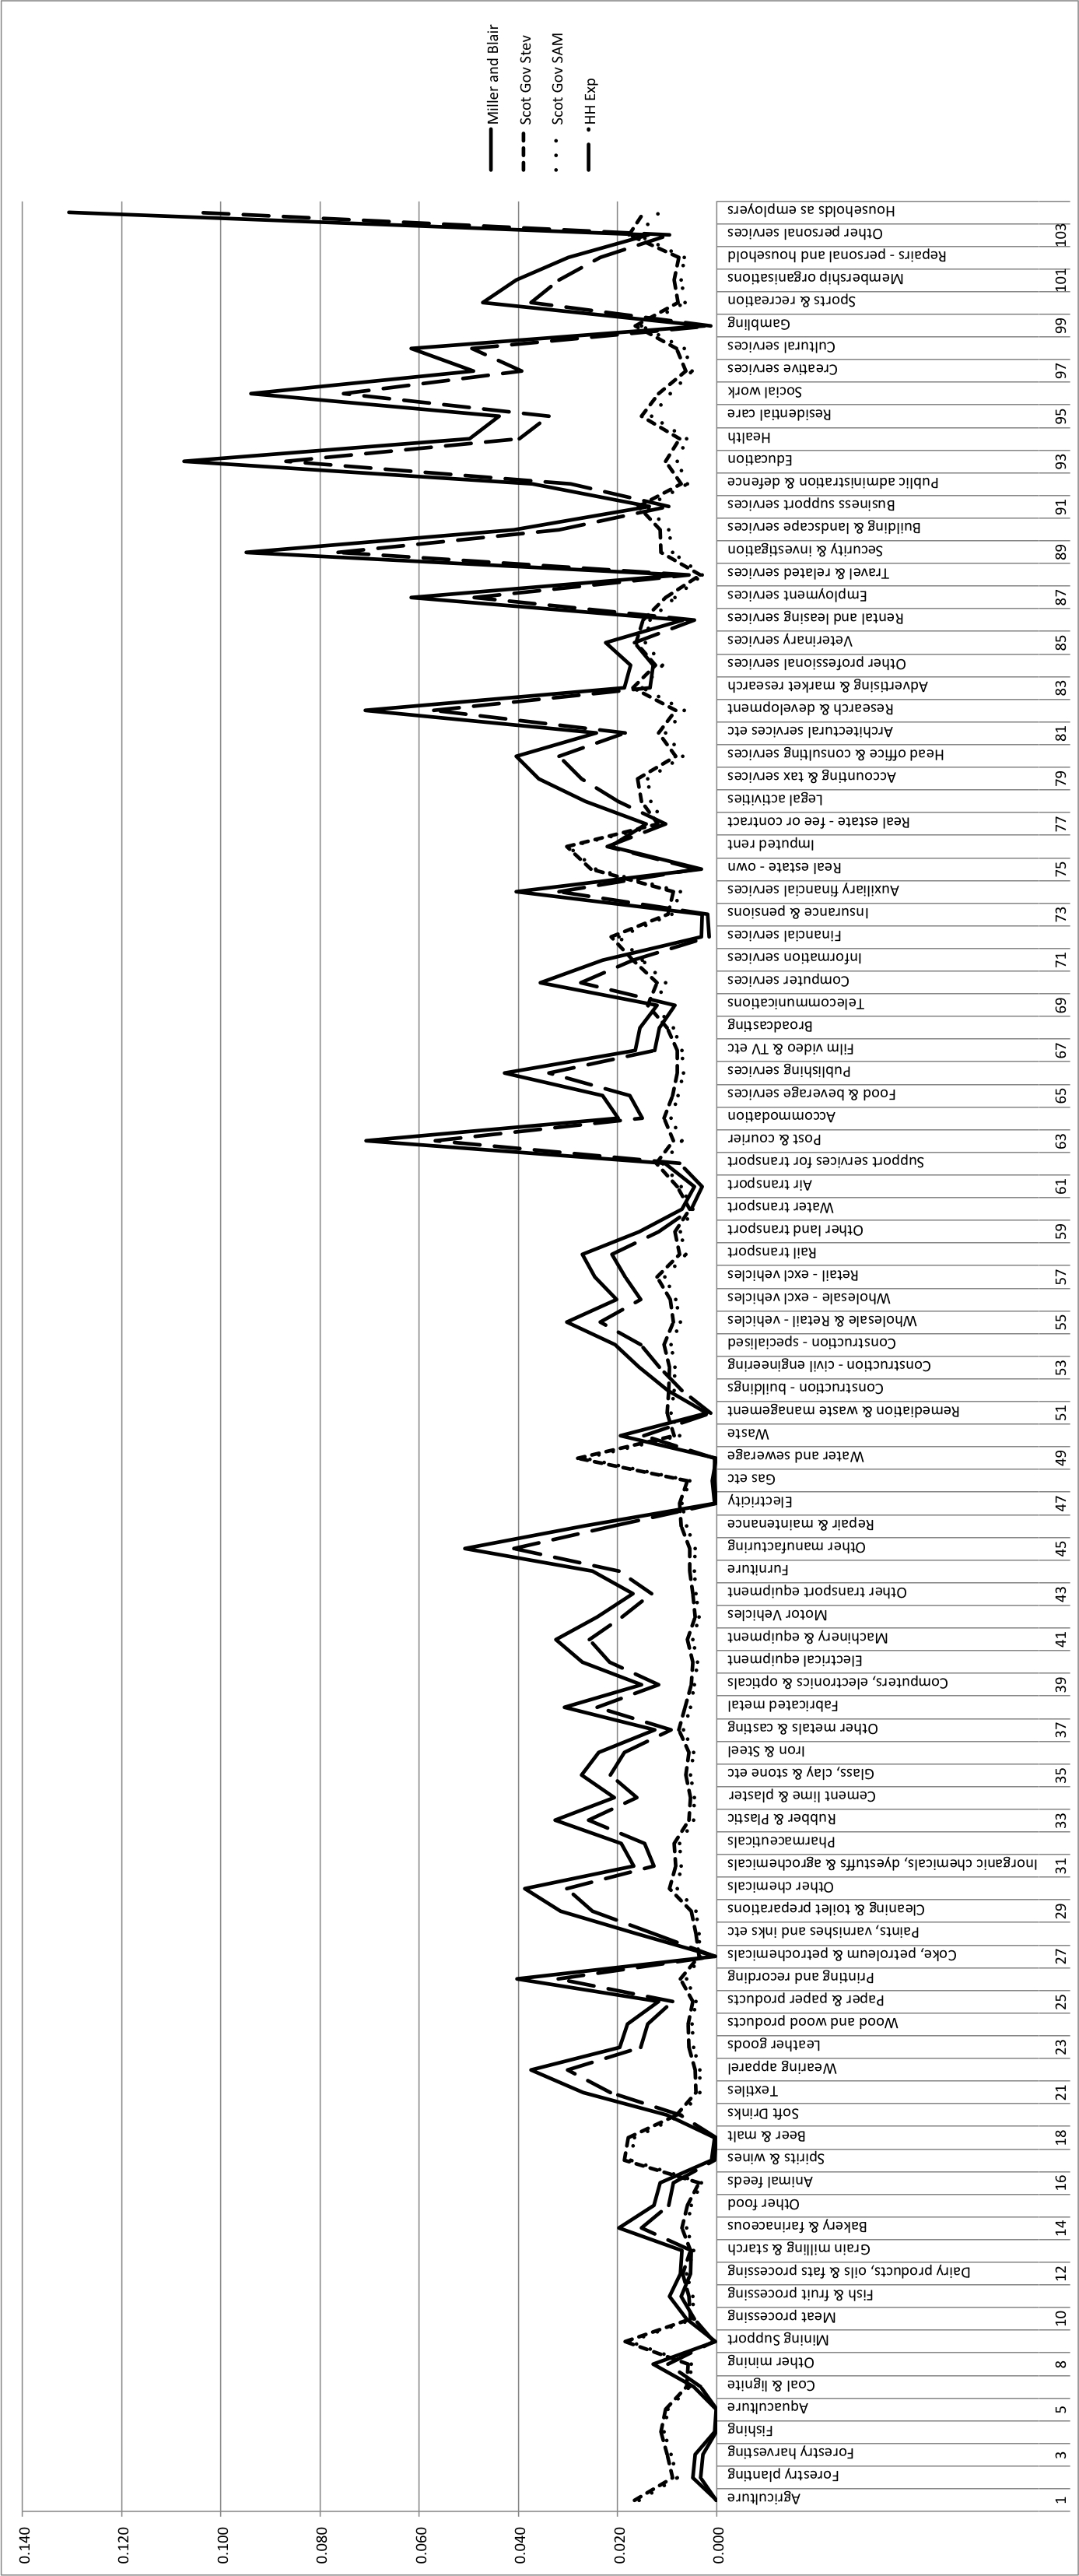
\includegraphics[width=3in]{DifferencesChart}
  \caption{Differences}
\end{figure}
 
% etc

%----------------------------------------------------------------------------------------
%	APPENDICES
%----------------------------------------------------------------------------------------

%% Appendix A
\newpage 
\section{Appendix A} 
\label{sec:Appendix A}

%\begin{landscape}
{\scriptsize
\begin{center} 
\begin{longtable}{lrrrrrr} %{rrrrrrr} 
\caption*{QLFS Observation per Industry compared to FTE employment (2009)} \label{Appendix A} \\ \\ \toprule

          & \multicolumn{2}{c}{QLFS Observations} & \multicolumn{2}{c}{FTE Employment} & \multicolumn{2}{c}{Observations in \%} \bigstrut[b]\\
\cline{2-7}          & Male  & Female & Male  & Female & Male & Female \bigstrut[t]\\

\hline \endfirsthead \multicolumn{2}{l}%
{{\bfseries \tablename\ \thetable{} -- continued from previous page}} \\\toprule

          & \multicolumn{2}{c}{QLFS Observations} & \multicolumn{2}{c}{FTE Employment} & \multicolumn{2}{c}{Observations in \%} \bigstrut[b]\\
\cline{2-7}          & Male  & Female & Male  & Female & Male & Female \bigstrut[t]\\

\hline \endhead \bottomrule \multicolumn{2}{l}{{Continued on next page}} \\ 
\endfoot \bottomrule \endlastfoot
     1. Agriculture & 419   & 105   & 33,959 & 7,307 & 1.23  & 1.43 \\
    2. Forestry planting & 55    & 3     & 1,448 & 414   & 3.76  & 0.60 \\
    3. Forestry harvesting & 23    & 6     & 2,059 & 990   & 1.12  & 0.61 \\
    4. Fishing & 47    & 1     & 2,375 & 456   & 1.98  & 0.22 \bigstrut[b]\\
     \hdashline[1pt/1pt]
    5. Aquaculture & 30    & 6     & 2,115 & 345   & 1.42  & 1.74 \bigstrut[t]\\
    6. Coal \& lignite & 19    & 2     & 1,353 & 29    & 1.40  & 6.93 \\
    7. Oil \& gas extraction, metal ores & 116   & 12    & -     & -     & -     & - \\
    8. Other mining & 33    & 3     & 2,636 & 229   & 1.23  & 1.31 \bigstrut[b]\\
     \hdashline[1pt/1pt]
    9. Mining Support & 366   & 86    & 18,018 & 2,499 & 2.03  & 3.42 \bigstrut[t]\\
    10. Meat processing & 61    & 25    & 4,202 & 1,773 & 1.44  & 1.38 \\
    11. Fish \& fruit processing & 79    & 37    & 5,427 & 3,085 & 1.46  & 1.20 \\
    12. Dairy products, oils \& fats processing & 21    & 12    & 2,445 & 625   & 0.86  & 1.84 \bigstrut[b]\\
     \hdashline[1pt/1pt]
    13. Grain milling \& starch & 6     & 3     & 207   & 69    & 2.90  & 3.62 \bigstrut[t]\\
    14. Bakery \& farinaceous & 47    & 50    & 6,982 & 4,607 & 0.67  & 1.07 \\
    15. Other food & 31    & 22    & 2,206 & 1,440 & 1.38  & 1.53 \\
    16. Animal feeds & 15    & 35    & 576   & 240   & 2.60  & 14.38 \bigstrut[b]\\
     \hdashline[1pt/1pt]
    17. Spirits \& wines & 73    & 28    & 6,581 & 2,958 & 1.11  & 0.93 \bigstrut[t]\\
    18. Beer \& malt & 23    & 8     & 557   & 227   & 4.13  & 3.30 \\
    19. Soft Drinks & 14    & 35    & 1,506 & 367   & 0.93  & 9.53 \\
    20. Tobacco & -     & -     & -     & -     & -     & - \bigstrut[b]\\
     \hdashline[1pt/1pt]
    21. Textiles & 27    & 17    & 4,300 & 2,464 & 0.62  & 0.67 \bigstrut[t]\\
    22. Wearing apparel & 10    & 21    & 1,543 & 2,638 & 0.65  & 0.80 \\
    23. Leather goods & 7     & 4     & 418   & 174   & 1.56  & 2.31 \\
    24. Wood and wood products & 77    & 9     & 6,960 & 824   & 1.10  & 1.03 \bigstrut[b]\\
     \hdashline[1pt/1pt]
    25. Paper \& paper products & 41    & 23    & 4,189 & 1,252 & 0.98  & 1.84 \bigstrut[t]\\
    26. Printing and recording & 79    & 19    & 4,099 & 1,636 & 1.92  & 1.16 \\
    27. Coke, petroleum \& petrochemicals & 69    & 5     & 2,275 & 400   & 3.03  & 1.25 \\
    28. Paints, varnishes and inks etc & 8     & 7     & 298   & 78    & 2.69  & 9.02 \bigstrut[b]\\
     \hdashline[1pt/1pt]
    29. Cleaning \& toilet preparations & 7     & 6     & 442   & 349   & 1.47  & 1.72 \bigstrut[t]\\
    30. Other chemicals & 6     & 3     & 1,358 & 876   & 0.44  & 0.34 \\
    31. Inorganic chemicals, dyestuffs \& agrochemicals & 4     & 3     & 1,041 & 204   & 0.34  & 1.22 \\
    32. Pharmaceuticals & 49    & 31    & 1,402 & 928   & 3.50  & 3.29 \bigstrut[b]\\
     \hdashline[1pt/1pt]
    33. Rubber \& Plastic & 123   & 20    & 6,880 & 1,362 & 1.79  & 1.43 \bigstrut[t]\\
    34. Cement lime \& plaster & 22    & 3     & 2,111 & 255   & 1.02  & 1.18 \\
    35. Glass, clay \& stone etc & 15    & 8     & 3,016 & 367   & 0.50  & 2.18 \\
    36. Iron \& Steel & 54    & 13    & 952   & 89    & 5.67  & 14.12 \bigstrut[b]\\
     \hdashline[1pt/1pt]
    37. Other metals \& casting & 8     & 2     & 855   & 92    & 0.94  & 2.16 \bigstrut[t]\\
    38. Fabricated metal & 205   & 28    & 23,823 & 3,142 & 0.86  & 0.89 \\
    39. Computers, electronics \& opticals & 143   & 52    & 8,791 & 3,286 & 1.63  & 1.57 \\
    40. Electrical equipment & 29    & 234   & 3,654 & 1,189 & 0.79  & 19.68 \bigstrut[b]\\
     \hdashline[1pt/1pt]
    41. Machinery \& equipment & 212   & 43    & 13,335 & 2,435 & 1.59  & 1.75 \bigstrut[t]\\
    42. Motor Vehicles & 88    & 6     & 2,225 & 226   & 3.96  & 2.66 \\
    43. Other transport equipment & 199   & 15    & 10,126 & 968   & 1.97  & 1.55 \\
    44. Furniture & 16    & 6     & 2,250 & 367   & 0.71  & 1.50 \bigstrut[b]\\
     \hdashline[1pt/1pt]
    45. Other manufacturing & 32    & 41    & 4,013 & 2,687 & 0.80  & 1.53 \bigstrut[t]\\
    46. Repair \& maintenance & 282   & 29    & 9,735 & 1,499 & 2.89  & 1.93 \\
    47. Electricity & 118   & 79    & 8,618 & 3,488 & 1.37  & 2.26 \\
    48. Gas etc & 65    & 21    & 5,135 & 596   & 1.27  & 3.44 \bigstrut[b]\\
     \hdashline[1pt/1pt]
    49. Water and sewerage & 73    & 25    & 4,291 & 919   & 1.69  & 2.66 \bigstrut[t]\\
    50. Waste & 117   & 14    & 8,607 & 1,245 & 1.36  & 1.08 \\
    51. Remediation \& waste management & 41    & 8     & 93    & 36    & 43.98 & 22.32 \\
    52. Construction - buildings & 958   & 148   & 43,029 & 7,737 & 2.23  & 1.91 \bigstrut[b]\\
     \hdashline[1pt/1pt]
    53. Construction - civil engineering & 412   & 67    & 25,954 & 2,449 & 1.59  & 2.72 \bigstrut[t]\\
    54. Construction - specialised & 1,073 & 71    & 81,351 & 10,009 & 1.32  & 0.70 \\
    55. Wholesale \& Retail - vehicles & 505   & 86    & 36,563 & 6,980 & 1.38  & 1.22 \\
    56. Wholesale - excl vehicles & 545   & 227   & 54,353 & 20,233 & 1.00  & 1.12 \bigstrut[b]\\
     \hdashline[1pt/1pt]
    57. Retail - excl vehicles & 963   & 1,455 & 76,822 & 112,984 & 1.25  & 1.29 \bigstrut[t]\\
    58. Rail transport & 60    & 4     & 5,247 & 1,170 & 1.13  & 0.34 \\
    59. Other land transport & 650   & 101   & 39,498 & 5,727 & 1.65  & 1.75 \\
    60. Water transport & 91    & 23    & 1,837 & 732   & 4.95  & 3.07 \bigstrut[b]\\
     \hdashline[1pt/1pt]
    61. Air transport & 45    & 7     & 2,358 & 1,626 & 1.91  & 0.43 \bigstrut[t]\\
    62. Support services for transport & 196   & 70    & 22,373 & 6,002 & 0.88  & 1.17 \\
    63. Post \& courier & 240   & 59    & 14,035 & 3,773 & 1.71  & 1.56 \\
    64. Accommodation & 209   & 276   & 22,143 & 25,102 & 0.94  & 1.10 \bigstrut[b]\\
     \hdashline[1pt/1pt]
    65. Food \& beverage services & 463   & 537   & 39,508 & 51,835 & 1.17  & 1.04 \bigstrut[t]\\
    66. Publishing services & 98    & 37    & 4,666 & 3,877 & 2.09  & 0.94 \\
    67. Film video \& TV etc & 27    & 24    & 2,031 & 2,386 & 1.30  & 0.98 \\
    68. Broadcasting & 21    & 28    & 548   & 419   & 3.84  & 6.68 \bigstrut[b]\\
     \hdashline[1pt/1pt]
    69. Telecommunications & 133   & 55    & 15,399 & 6,313 & 0.86  & 0.87 \bigstrut[t]\\
    70. Computer services & 263   & 64    & 20,672 & 7,860 & 1.27  & 0.81 \\
    71. Information services & 12    & 11    & 1,461 & 772   & 0.79  & 1.42 \\
    72. Financial services & 242   & 353   & 18,930 & 26,124 & 1.28  & 1.35 \bigstrut[b]\\
     \hdashline[1pt/1pt]
    73. Insurance \& pensions & 124   & 167   & 9,200 & 9,375 & 1.35  & 1.78 \bigstrut[t]\\
    74. Auxiliary financial services & 187   & 157   & 10,704 & 11,954 & 1.75  & 1.31 \\
    75. Real estate - own & 65    & 86    & 7,077 & 9,098 & 0.91  & 0.94 \\
    76. Imputed rent & -     & -     & -     & -     & -     & - \bigstrut[b]\\
     \hdashline[1pt/1pt]
    77. Real estate - fee or contract & 19    & 57    & 4,771 & 5,046 & 0.39  & 1.12 \bigstrut[t]\\
    78. Legal activities & 95    & 120   & 5,608 & 14,710 & 1.69  & 0.82 \\
    79. Accounting \& tax services & 88    & 101   & 13,400 & 21,140 & 0.65  & 0.48 \\
    80. Head office \& consulting services & 92    & 73    & 9,777 & 8,298 & 0.94  & 0.88 \bigstrut[b]\\
     \hdashline[1pt/1pt]
    81. Architectural services etc & 555   & 168   & 41,951 & 14,439 & 1.32  & 1.16 \bigstrut[t]\\
    82. Research \& development & 75    & 87    & 4,521 & 3,509 & 1.66  & 2.46 \\
    83. Advertising \& market research & 34    & 15    & 3,275 & 2,452 & 1.02  & 0.61 \\
    84. Other professional services & 108   & 57    & 5,580 & 3,822 & 1.93  & 1.49 \bigstrut[b]\\
     \hdashline[1pt/1pt]
    85. Veterinary services & 13    & 35    & 390   & 3,032 & 3.21  & 1.14 \bigstrut[t]\\
    86. Rental and leasing services & 98    & 44    & 12,044 & 3,403 & 0.81  & 1.29 \\
    87. Employment services & 83    & 99    & 25,726 & 16,892 & 0.32  & 0.58 \\
    88. Travel \& related services & 36    & 59    & 2,099 & 5,085 & 1.69  & 1.15 \bigstrut[b]\\
     \hdashline[1pt/1pt]
    89. Security \& investigation & 187   & 24    & 10,111 & 1,554 & 1.85  & 1.54 \bigstrut[t]\\
    90. Building \& landscape services & 281   & 182   & 30,450 & 27,219 & 0.92  & 0.67 \\
    91. Business support services & 95    & 148   & 11,606 & 11,157 & 0.81  & 1.32 \\
    92. Public administration \& defence & 1,111 & 1,022 & 69,710 & 72,334 & 1.59  & 1.41 \bigstrut[b]\\
%     \hdashline[1pt/1pt]
    93. Education & 804   & 2,057 & 52,278 & 108,300 & 1.54  & 1.90 \bigstrut[t]\\
    94. Health & 572   & 1,817 & 38,305 & 141,342 & 1.49  & 1.29 \\
    95. Residential care & 236   & 628   & 11,759 & 43,057 & 2.00  & 1.46 \\
    96. Social work & 241   & 997   & 14,785 & 58,784 & 1.63  & 1.70 \bigstrut[b]\\
     \hdashline[1pt/1pt]
    97. Creative services & 81    & 75    & 2,737 & 2,246 & 2.96  & 3.32 \bigstrut[t]\\
    98. Cultural services & 43    & 86    & 4,680 & 6,699 & 0.92  & 1.28 \\
    99. Gambling & 37    & 44    & 2,506 & 4,528 & 1.46  & 0.96 \\
    100. Sports \& recreation & 253   & 147   & 17,875 & 12,648 & 1.42  & 1.16 \bigstrut[b]\\
     \hdashline[1pt/1pt]
    101. Membership organisations & 124   & 111   & 7,807 & 11,491 & 1.59  & 0.97 \bigstrut[t]\\
    102. Repairs - personal and household & 103   & 21    & 2,119 & 993   & 4.86  & 2.11 \\
    103. Other personal services & 76    & 308   & 8,713 & 14,025 & 0.87  & 2.19 \\
    104. Households as employers & 6     & 15    & 476   & 1,149 & 1.26  & 1.26 \\
    \hline
    \multicolumn{1}{l}{Total} & 16,813 & 13,958 & 1,212,308 & 1,017,623 & 1.39 & 1.37  \\
    \end{longtable}
\end{center} 
} %\end{landscape}

Note: 

\bigskip

Total FTE QLFS sample comprises of 30,0771 observations. 16,813 thereof are male and 13,958 are female. Total Scottish FTE employment is 2,229,931 of which 1,212,308 are male and 1,017,623 are female. The QLFS sample covers 1.37 percent of total FTE employment, 1.39 percent of total male FTE employment and 1.37 percent of total female FTE employment. Summary statistics of the QLS sample are summarised in the following table:

\bigskip

\begin{table}[H] \caption*{Summary statistics of QLFS sample}
\bigskip \begin{scriptsize} \begin{centering} \begin{doublespacing}
% INSERT
    \begin{tabular}{lrrrr}
   \toprule
          & Mean  & Median & Minimum & Maximum \\
    Male  & 161.659 & 76.0000 & 0.0000 & 1111.00 \\
    Female & 134.212 & 34.5000 & 0.0000 & 2056.50 \\
          & Std. Dev. & C.V.  & Skewness & Ex. kurtosis \\
    Male  & 232.807 & 1.4401 & 2.4613 & 5.8950 \\
    Female & 330.637 & 2.4636 & 4.2134 & 18.3198 \\
          & 5\% Perc. & 95\% Perc. & IQ range & Missing obs. \\
    Male  & 6.0000 & 765.5000 & 171.1250 & 0.0000 \\
    Female & 2.1250 & 904.3750 & 75.1250 & 0.0000 \\
% INSERT END  
\bottomrule \end{tabular}%  
\begin{flushright}  \end{flushright} 
\end{doublespacing} \end{centering} \end{scriptsize} \end{table} \bigskip


 
% etc
%----------------------------------------------------------------------------------------
%	BIBLIOGRAPHY
%----------------------------------------------------------------------------------------

\newpage 
\begin{spacing}{2.3}
\interlinepenalty=10000
\bibliography{references}
\newpage
\pagenumbering{roman}
\thispagestyle{empty}
\mbox{}
\newpage
\end{spacing}

%----------------------------------------------------------------------------------------
%	END
%----------------------------------------------------------------------------------------


\end{document}